\documentclass[11pt]{report}
\usepackage[portuguese]{babel}
\usepackage[utf8]{inputenc}
%\usepackage[dvips]{graphicx}
\usepackage{graphicx}
\usepackage{enumitem}
\usepackage[normalem]{ulem}
\usepackage{latexsym}
\usepackage{amsmath}
%\usepackage{hyperref}

\newcounter{qcounter}

\setlength{\parindent}{0pt}
\setlength{\parskip}{3ex plus 0.5ex minus 0.5ex}

\addtolength{\voffset}{-0.8cm}
\addtolength{\textheight}{1.6cm}
\addtolength{\hoffset}{-1.0cm}
\addtolength{\textwidth}{2.0cm}

\pagestyle{plain}

% =============== Seção de definições de macros ========================

% Delimita uma seção:
\newenvironment{secao}[1] {
    \framebox[\textwidth] {
        \rule[-1.2ex]{5ex}{5.5ex}
        {\Large\sf #1}
        \hspace{\stretch{1}}
    } \addcontentsline{toc}{chapter}{#1}
    %\begin{sf}
    \nopagebreak[4]
} { 
    %\end{sf}
}


% Delimita uma subseção 
\newenvironment{subsecao}[1] {
    \rule[0ex]{2.5ex}{2.5ex}
    {\Large\sf #1}
	 \addcontentsline{toc}{section}{#1}
    \nopagebreak[4]
}{ }

% Coloca uma figura (sem ser quadrinhos)
\newcommand{\figura}[1] {
    \begin{figure}[!htbp]
      \begin{center}
        \includegraphics[width=\textwidth]{imagens/#1.pdf}
      \end{center}
    \end{figure}
}

% Coloca quadrinhos
\newcommand{\quadrinhos}[1] {
    \figura{quad#1}
}


% ============================ Documento ===============================
\begin{document}

%Renomeando o índice------------------------------------------------------------
%\renewcommand{\contentsname}{\center Não se perca, bixo...}
\renewcommand{\contentsname}{\center Esse guia contém...}

% Capa -------------------------------------------------------------------------
\figura{capa}
\clearpage
\pagebreak

% Coloca o índice --------------------------------------------------------------
\tableofcontents
\newpage

% Editorial --------------------------------------------------------------------
\begin{secao}{Editorial}

Bixo (opa, bixo é com letra minúscula), foi difícil chegar até aqui. Você está
meio ou completamente perdido. Temos apenas uma sugestão: aproveite esta etapa.
Faça da sua estadia na USP o melhor tempo da sua vida. Você verá que a USP tem
muitas e muitas coisas a oferecer. Não se preocupe apenas em estudar e passar de
ano, como você fez durante sua vida inteira; aproveite TUDO (você ainda vai
descobrir a definição de TUDO). Você pode não acreditar nisto agora, mas saiba
que viverá momentos inesquecíveis aqui no IME, alguns fantásticos e outros deploráveis. 

Este guia foi feito para você, bixo que já sabe ler (se não souber, apenas olhe
as figuras), possa aprender um pouquinho do que é a USP, o IME e a vida de
universitário que se inicia agora. Ele foi escrito numa forma descontraída e
fácil para que você consiga entender; mesmo assim, se pintar alguma dúvida,
você pode se dirigir a qualquer VETERANO, e sua dúvida será sanada (e, quem sabe,
talvez você também comece uma nova e forte amizade). Outra coisa: LEIA E DECORE
COMPLETAMENTE ESTE GUIA PARA NÃO PAGAR MICO. Pensando bem, você vai pagar mico
de qualquer jeito; ainda assim, seja um mínimo precavido e leia-o.

Lembre-se: este é seu último ano como bixo. Aproveite!

\vspace{\stretch{1}}
\rule{\textwidth}{0.5ex}\rule{2ex}{0.5ex}

\begin{small}
\begin{tabular}{|p{\textwidth}|}
\hline
\\[0.2pt]
{\large\bf Guia do bixo 2013} \\
Uma publicação da Comissão de Trote \\
\\
\makebox[4cm][l]{{\bf Editores}} Arthur, David, Godinez e Luiz\\
%
%\makebox[4cm][l]{{\bf Capa}} David e Wil-Kazuo.\\ %FIXME Arrumar após fazer a capa
%
\makebox[4cm][l]{{\bf Textos}} André Verri (Deco), Antonieta, Fábio da Yumi, Gizela Fonseca,\\
\makebox[4cm][l]{{\bf       }} Lucas Cavalcanti, Marina Trindade, Mauricio Camilo,\\
\makebox[4cm][l]{{\bf       }} Paula Corradi, Pedrosa, Pedrão, Renata Aguemi,\\ 
\makebox[4cm][l]{{\bf       }} Ricardo Yasuda,  Yumi, David, Wil-Kazuo e autores dos textos\\ 
\makebox[4cm][l]{{\bf       }} dos guias anteriores não supracitados.\\
%
\makebox[4cm][l]{{\bf Layout}} btco (Guia 2007)                          \\
\makebox[4cm][l]{{\bf Revisão geral}} Dado a falta de tempo, bixo, a revisão é com você!\\
\makebox[4cm][l]{{\bf Agradecimentos:}} \\

$\qquad\qquad$Ao Donald Knuth (por inventar o \TeX\makebox{} e salvar-nos do Word na preparação
desse guia), ao btco pela iniciativa de começar este guia em \LaTeX\makebox{},
ao gimp por nos ajudar a editar as figuras, aos bixos por lerem o guia todo
e decorarem as músicas e os dez mandamentos e aos organizadores dos guias anteriores,
afinal nada se cria, tudo se copia. Por último, à gráfica e às pessoas da Comissão
que perderam as férias para que este guia ficasse pronto.\\
\makebox[4cm][l]{{\bf       }}                                            \\
\hline
\end{tabular}
\end{small}

\pagebreak

\begin{subsecao}{Os Dez Mandamentos}
  \begin{enumerate}
  \item O VETERANO tem sempre razão;
  \item Na improvável hipótese de o bixo ter razão, entra imediatamente
        em vigor o primeiro mandamento;
  \item Em qualquer evento social, as despesas correm sempre por conta
        do bixo;
  \item O bixo tem o direito de permanecer calado (exceto quando interpelado
        por um VETERANO). Tudo o que disser pode e será usado contra ele;
  \item O bixo deve se apresentar imediatamente em caso de convocação por
        um VETERANO. Os desertores serão severamente punidos;
  \item Não são válidos no IME os direitos constitucionais do bixo à vida,
        liberdade e igualdade;
  \item O bixo deve estar pronto para assumir as seguintes funções para um
        VETERANO: cadeira, cinzeiro, moleque de recados, etc, quando as
        circunstâncias assim o exigirem; e também quando não o exigirem.
  \item O bixo deve amar respeitar e os seus VETERANOS acima de qualquer
        coisa;
  \item Para os casos não abrangidos por estas regras, a decisão final
        correrá por conta dos VETERANOS.
  \item Todo bixo é BURRO.
  \end{enumerate}

  
Como bixo, você tem todo o direito de reclamar sobre os mandamentos! Qualquer
reclamação deverá ser protocolada em três vias datadas, assinadas e autenticadas,
com firma reconhecida em cartório, e assim encaminhada à Comissão de Trote 2013
via mala direta. As reclamações serão incineradas e os reclamantes severamente
punidos. Obs.: alguns VETERANOS sugeriram que incinerássemos os reclamantes também.
A medida está em estudo, devido ao custo da operação e ao lixo tóxico produzido.


\end{subsecao}
\end{secao}

\pagebreak

% Carta Aos Ingressantes -------------------------------------------------------
\begin{secao}{Carta Aos Ingressantes}

Agora que vocês entraram na USP, bixos, vocês adquiriram novas
responsabilidades.  Vocês são responsáveis por si mesmos, isto é, ninguém irá se
preocupar com seus problemas acadêmicos (matrículas, notas erradas, dificuldade
com algumas matérias, rixa com professores, etc.) se vocês mesmos não se
preocuparem. Existem pessoas que poderão ajudá-los, mas só o farão se vocês
forem procurá-las. Caso contrário, os únicos prejudicados serão vocês.

A faculdade não é o Paraíso (essa estação fica na Avenida Paulista), mas pode
melhorar a cada dia. Nós, alunos, também devemos contribuir para essa melhora.
Vocês são o futuro da universidade. Portanto, participem, reclamem, busquem seus
direitos, ajudem e, principalmente, não tenham medo de cara feia, pois isso é o
que não vai faltar.

Lembrem-se que vocês não são mais crianças e já sabem o que querem sem que
outros precisem decidir por você; então procurem o que lhes interessa: iniciação
científica, estágios, monitorias, matérias que não são obrigatórias mas que
vocês gostariam de fazer (mesmo que não tenha nada a ver com seu curso);
participação no CAMat ou na Atlética, esportes no CEPE, artigos no jornal, etc.,
etc., etc.

Vocês não são mais crianças, mas também não são o bambambã; então lembrem que
seus amigos vão ser muito importantes para vocês e para o bom andamento do seu
curso. Procurem combinar atividades fora da faculdade, diferentes do cotidiano,
porque isso ajuda a amenizar o estresse que o dia a dia na faculdade pode
trazer.

Além de tudo, vocês não podem se esquecer de uma parte importante de suas vidas
universitárias, que é estudar. Tentem não deixar para estudar na véspera da
prova porque a probabilidade de vocês não irem bem é bem alta (exceto se vocês
tiverem uma sala do tempo em casa, que nem a do Dragon Ball). A mesma coisa se
aplica aos EPs, ainda mais que, quanto mais próximo da data de entrega, mais
erros vão aparecer e, na maioria dos casos, os EPs não são aceitos depois da
data limite de entrega e, caso sejam aceitos, não valerão a mesma nota.

Além disso, como em todo lugar, existem aquelas pessoas ranzinzas e pentelhas
que acham super bacana acabar com a graça de todo mundo, criticar o IME e
aumentar a sua baixo-estima dizendo que os cursos são impossíveis e que vocês
não vão se formar nunca, mas não acreditem neles, vocês entraram aqui com um
propósito. Sigam-no.

Obs.: Esse guia é autoexplicativo; portanto, não se assustem com palavras e
siglas que vocês não entenderam. Continuem lendo, porque tudo será explicado em
detalhes, mastigado, tim-tim por tim-tim. Saibam que vai faltar um monte de
siglas...  Aprendam-nas seletiva e rapidamente. Destaques para: USP, IME, MAC,
MAT, MAE, MAP, BCC, BM, BMA, LIC, BMAC, BE, CEPE, CEAGESP, CTA, RD, CAMat,
AAAMat, SSG, PUTUSP, P1, P2, P3, P4, P5, Pn, PQP, CEC, CNPq (=\$), FAPESP
(=\$\$\$), CG, DP, REC, SUB (esta última, ou talvez as duas ou três últimas,
vocês vão conhecer bem melhor, mais cedo ou mais tarde).

\end{secao}

\pagebreak

% Comissão de Trote e o Kit-bixo -----------------------------------------------
\quadrinhos1
\begin{secao}{Comissão de Trote e \textit{Kit}-bixo}

A Comissão de Recepção aos Calouros, também conhecida como Comissão de Trote, é
responsável por auxiliar os ingressantes em seus primeiros momentos imeanos.
Sabemos que não é um momento fácil. Vocês estão entrando em uma nova fase de
suas vidas, em um lugar estranho, com pessoas estranhas (em todos os sentidos),
e nosso objetivo é fazer com que vocês se sintam bem-vindos e se integrem
($\int$) com seus coleguinhas e seus VETERANOS!

Vocês já devem ter conhecido alguns de nós durante a matrícula, aquelas pessoas
bem legais que estavam devidamente uniformizadas, cuidando para que nenhum
bêbado ou pessoa de má índole machucasse vocês! Parte da Comissão ajuda os
alunos a preencher os formulários e a se matricular direitinho. Enquanto isso,
outra parte impede que a espera na fila de matrícula seja tediosa e confusa:
todos os bixos são devidamente pintados, carimbados e tosados, numa tentativa
de torná-los mais charmosos. Duro esse trabalho, não?

A Comissão de Trote organiza a super Semana de Recepção, cheia de atividades
legais! (Vocês devem ter recebido, junto com aquela papelada na matrícula, a
programação da Semana. Se não receberam, procurem arrumar uma, logo!).
E adivinhem quem organiza o magnífico encontro dos bixos: IMEntrando, que deverá
ocorrer no dia 2 de abril. Não esqueçam essa data, bixos! %REFTIME

A Comissão de Trote é formada pelos mais animados e divertidos VETERANOS. Como
dissemos, eles organizam a matrícula, agilizam a papelada, mantêm um clima
alegre na recepção, fazem isso e aquilo na Semana de Recepção...
Vocês devem estar pensando ``Puxa! Como nós, bixos, podemos retribuir
tamanha dedicação?'' É simples, bixos: {\bf\em comprem o \textit{kit}-bixo}!!!

O \textit{kit}-bixo, como vocês devem saber, é um conjunto de coisas
importantíssimas para vocês, ingressantes perdidos! Ele contém dois tipos de
itens:
\begin{itemize}
\item itens úteis;
\item itens essenciais.
\end{itemize} %REFTIME (Isso muda todo ano)
Dentre eles temos uma camiseta, que serve para que nós os identifiquemos como
bixos e para que as pessoas na rua achem que vocês são inteligentes (fiquem
tranquilos, bixos, vocês não são tão melhores assim); materiais personalizados
com o símbolo do IME pra vocês usarem nas aulas e mostrarem a seus amigos; uma
caneca (também personalizada), pra vocês economizarem muitos copos no bandejão e
que ainda serve como convite para o IMEntrando; dois adesivos pra vocês, um para
vocês colarem no carro que vão ganhar de presente, e outro para os papais
(quando vocês virem o adesivo vocês vão entender); calculadora para usarem nas
suas provas de Estatística; um squeeze pra aguentarem o calor do começo do ano;
duas tatuagem personalizadas para mostrarem o amor pelo IME em suas peles; um
pendrive de 8GB, para vocês guardarem todos os arquivos e EPs das matérias; um
caderno personalizado feito com muito \sout{suor} carinho pela Comissão. Todas
essas coisas contidas em uma mochila sport do IME-USP, afinal não dá pra
carregar tudo isso na mão, né?

Adquiram o maravilhoso \textit{kit}-bixo do IME-USP. Ele estará à venda na
matrícula e na semana de recepção, até durarem os estoques. (Não vão chorar
depois, hein?)

Para terminar, além de tudo isso, a Comissão é que faz esse maravilhoso guia que
vocês estão lendo agora (ou estão só olhando as figuras, vai
saber...). Esperamos que vocês gostem do nosso trabalho! Qualquer coisa, nos
procure! Entrem na nossa página no Facebook: {\tt fb.com/troteimeusp} contando o
que vocês sentiram ao ler o guia, o que fizeram com vocês na matrícula (com o
nome do VETERANO na denúncia), o que vocês acharam da semana de recepção e se
vocês se sentiram bem-vindos ou querem voltar logo para perto da sua
mãe. Estaremos sempre prontos a ajudá-los!
\end{secao}


% O CAMat ----------------------------------------------------------------------
\begin{secao}{O CAMat}

O Centro Acadêmico da Matemática, Estatística e Computação é o que chamamos de
CAMat. É um órgão reconhecido pelo IME, feito pelos estudantes e para os
estudantes.

É dever do CAMat lutar pelos nossos direitos, organizando debates, palestras,
além, é claro, de eventos culturais, encontros, feiras de livros, festas...

O CAMat representa os alunos junto ao IME e todas as demais entidades do nosso
Instituto. O CAMat não é simplesmente uma sala, um espaço. O CAMat somos nós,
todos os alunos do IME, anualmente representados por um grupo de alunos que
vence um pleito democrático, do qual você também participará, seja votando ou,
logo, logo, sendo votado!

Todas as atividades promovidas pelo CAMat são discutidas e decididas em
reuniões, nas quais, pelo menos desde a gestão 2010, todo aluno do IME tem
direito a voz e voto. Elas serão a melhor oportunidade para você apresentar suas
ideias, questionar, ou simplesmente ficar a par do que o CAMat
anda fazendo.

A sala do CAMat  fica dentro da Vivência, na sala 18 do bloco B. Você tem acesso
livre lá dentro para conversar, ver TV, ler jornais e revistas, jogar sinuca,
pebolim, xadrez, BARALHO (aqui você vai aprender um número inimaginável de
jogos de baralho...)\footnote{Veja a seção desse guia dos jogos da
Vivência} e até estudar.

Para salvar suas costas dos milhares de livros de defesa contra as artes das
Trevas (Cálculo, Álgebra, Análise...) que você precisará carregar, o CAMat
também aluga armários aos alunos a uma taxa insignificante. Fique atento, pois no
início das aulas do 1º semestre ocorrerá a renovação dos armários com
aqueles alunos VETERANOS que já os têm e certamente sobrará uma boa quantidade
de armários para outros, incluindo vocês, bixos.

Além desses, o CAMat oferece alguns outros serviços:

\begin{itemize}
\item Organizamos um Banco de Provas, que contém várias provas dos anos anteriores feitas
pelos maravilhosos VETERANOS. Não se esqueça de contribuir com sua prova também.
\item Emprestamos baralhos, violões e fichas de pôquer mediante apresentação de
carteirinha USP.
\item Em seus momentos de fome e sede fique tranquilo, pois no CAMat você
também encontra alguns "comes e bebes", prontos para matar aquela fome e sede
que teimam em aparecer praticamente a toda hora... Ah! Os preços são praticamente
de atacado!
\item Temos também uma máquina de café disponível a todos que queiram lutar
contra o sono... É só chegar lá e preparar, de graça!
\end{itemize}

Bom, mas o CAMat não é e nem deve ser feito só de serviços. Há atualmente
muitas mudanças no nosso instituto, e precisamos garantir que os alunos não
saiam prejudicados. Em 2010, trouxemos, junto com o
DCE, uma exposição sobre a ditadura militar para o saguão do IME. Para abrir a
exposição e discutir o assunto com a gente, recebemos o então Ministro dos
Direitos Humanos, Paulo Vannuchi. Achamos fundamental discutir assuntos não só
relativos ao IME, mas também à USP, ao Brasil e ao mundo.

%TODO Fazer esse próximo parágrafo usando o ambiente description, assim como
% na seção da Rede Linux.

O CAMat também tem uma página na web: \url{http://www.ime.usp.br/~camat}, um
e-mail: \url{camat.usp@gmail.com}, um grupo de e-mails \url{camat-aberto@googlegroups.com.br} (faça parte!), Facebook \url{fb.com/CAMatUSP} e Twitter \url{@camat_usp} e um telefone: 3091-6293, para você entrar em contato sempre
que precisar (quando roubarem seu lanche, puxarem seu cabelo ou te chamarem de
bobo).

LEMBRE: não deixe de participar (ao menos para conhecer) das reuniões do
CAMat. Local e horários serão propriamente divulgados.

LEMBRE$^2$: você é SEMPRE bem-vindo na salinha do CAMat.

\end{secao}


% A Atlética -------------------------------------------------------------------
\quadrinhos2
\begin{secao}{A Atlética} %REFTIME - Quase tudo aqui é REFTIME...

\begin{subsecao}{O que é a AAAMat?}

É a Associação Atlética Acadêmica da Matemática - a entidade mais divertida do
mundo!!!! - que tem como objetivo trazer os melhores momentos da sua vida
universitária! A atlética é formada por um grupo de IMEanos (gestão) que é
responsável por organizar atividades esportivas e eventos (festas, pizzadas,
premiações, etc) para a comunidade IMEana.

\end{subsecao}
%%%%%%%%%%%%%%%%%%%%%%%%%%%%%%%%%%%%%%%%%%%%%%%%%%%%%%%%%%%%%%%%%%%%%%%%%%%%%%%%

Algumas das atividades da Atlética:

\begin{subsecao}{Atividades esportivas internas:}

Na AAAMat existem diretores de modalidade (DMs) que são pessoas responsáveis
pelos treinos e campeonatos dos seguintes esportes: futebol de campo, futsal,
basquete, vôlei, handebol, atletismo, natação, tênis de mesa, tênis de campo,
xadrez, judô, beisebol, softbol, ultimate frisbee, bridge, rugby e e-sports
(\textit{League of Legends}, \textit{Hearthstone} e
\textit{Counter Strike: Global Offense}).

Os dias e horários dos treinos/jogos de cada uma dessas modalidades serão
sempre informados através do site e do mural da Atlética, localizado na entrada
do bloco B (aquele mural verde, colado na parede em frente a lanchonete).

Com essa variedade de modalidades, não tem desculpa pro sedentarismo hein,
bixo? Se você não conhece nenhuma delas, a gente te apresenta e se já conhece,
vem dar aquele “ooooi, sumido!!!” pra aquele esporte que você largou por conta
da fuvest! Ah, não esqueça de torcer pelos nossos atletas! Raça e coração, IME!

Além disso, a Atlética promove anualmente campeonatos internos daqueles jogos
que a gente passa hooooras fritando em casa. Já foram promovidos campeonatos de
Winning Eleven, LoL, Mario Kart, Super Smash Bros, Mario Tenis, Guitar Hero e
sinuca.

Ideias e sugestões sobre novas modalidades, campeonatos, inters, etc. são
sempre muito  bem-vindas! Conversem com a gente!

\end{subsecao}
%%%%%%%%%%%%%%%%%%%%%%%%%%%%%%%%%%%%%%%%%%%%%%%%%%%%%%%%%%%%%%%%%%%%%%%%%%%%%%%%

A AAAMat também representa o IME em diversos campeonatos universitários. São
eles:

\begin{subsecao}{BichUSP}

De nome intuitivo e charmoso, o BichUSP é um campeonato disputado entre as
faculdades da USP em que apenas os bixos (VOCÊS!) participam. O campeonato
acontece logo nas primeiras semanas de aula, sempre aos finais de semana. Aqui,
vocês têm a chance de suar a camisa IMEana pela primeira vez e ver a torcida
indo ao delírio em cada jogada - ganhando ou perdendo, seus veteranos estarão
vibrando por vocês!

%REFTIME
Esse ano o BichUSP acontecerá nas seguintes datas:

\begin{itemize}
  \item Tênis todos os dias do BichUSP
  \item 10 e 11/03/2018 - Basquete e Handebol.
  \item 17 e 18/03/2018 - Natação, Atletismo, Tênis de Mesa e Xadrez.
  \item 24 e 25/03/2018 - Futebol de campo e Rugby.
  \item 07 e 08/04/2018 - Vôlei e Futsal.
\end{itemize}

``Mas, Atlética, eu não sei jogar nenhum desses esportes :('' - Não tem
problema, a gente te ensina! Teremos treinos especiais para que vocês conheçam
a modalidade, os DM’s, os técnicos, a gente e os outros bixos que te
acompanharão nesse momento único da graduação!

Se você acha que tem alergia a esportes, dá uma chance da gente te mostrar o
contrário! São várias modalidades com várias dinâmicas diferentes, alguma delas
com certeza vai se encaixar no que você gosta! Se quiser só assistir no começo
e vir torcer com a gente, apareçam nos jogos que nós gritamos "VERMELHO E
BRANCO ATÉ MORRER" todos juntos!

Pra vocês se inspirarem, fizemos essa tabelinha que mostra quantos bixos
brilharam em anos anteriores. Estamos ansiosos pra completar ela com as
conquistas que virão esse ano:

%REFTIME
\begin{center}
  \begin{tabular}{c|c}
    \hline
    Ano & Campeão\\
    \hline
    2005 & Basquete Masculino \\
    2005 & Tênis de Mesa Feminino \\
    2007 & Atletismo Masculino\\
    2009 & Atletismo\\
    2011 & Tênis de Campo Feminino\\
    2012 & Basquete Feminino\\
    2014 & Tênis de Mesa Masculino\\
    2014 & Futsal Masculino\\
    2015 & Futsal Masculino\\
    2016 & Vôlei Masculino\\
    2017 & Xadrez, Rugby Misto e Rugby Feminino (IME+EFEE)\\
    2018 & Xadrez, Futebol de Campo F.\\
    2019 & VEM BIXES!
    \hline
  \end{tabular}
\end{center}

\end{subsecao}
%%%%%%%%%%%%%%%%%%%%%%%%%%%%%%%%%%%%%%%%%%%%%%%%%%%%%%%%%%%%%%%%%%%%%%%%%%%%%%%%
\begin{subsecao}{Copa USP}

A Copa USP é o primeiro campeonato após o BichUSP, e existem duas séries (Azul:
1º divisão e Laranja: 2º divisão). São nesses jogos que colocamos em prática
tudo o que fizemos nos treinos semanais para brilharmos nos jogos da fase de
grupos e então seguir arrasando nos jogos mata-matas.

\end{subsecao}
%%%%%%%%%%%%%%%%%%%%%%%%%%%%%%%%%%%%%%%%%%%%%%%%%%%%%%%%%%%%%%%%%%%%%%%%%%%%%%%%
\begin{subsecao}{Jogos da Liga}

Acontece no segundo semestre (UFA, já passou a P1 de cálculo, vem Cálculo 2!!!
\sout{Ou não}) e nessa competição não existe separação por séries. Somente as
faculdades da USP jogam e as disputas são sorteadas para formarem grupos e
então apenas os melhores colocados seguem para a fase final. Essa é a
oportunidade perfeita para gritar um "CHUPA POLI" na arquibancada.

\end{subsecao}
%%%%%%%%%%%%%%%%%%%%%%%%%%%%%%%%%%%%%%%%%%%%%%%%%%%%%%%%%%%%%%%%%%%%%%%%%%%%%%%%
\begin{subsecao}{NDU}

Esse campeonato acontece duas vezes ao ano, e várias faculdades de São Paulo
(tanto das USP quanto algumas não-usp) competem na cidade em busca dos melhores
resultados. Confira com o DM da modalidade se o time está participando da
competição.

\end{subsecao}
%%%%%%%%%%%%%%%%%%%%%%%%%%%%%%%%%%%%%%%%%%%%%%%%%%%%%%%%%%%%%%%%%%%%%%%%%%%%%%%%
\begin{subsecao}{BIFE}

O BIFE É O MELHOR EVENTO ESPORTIVO DO MUNDO! As iniciais das quatro fundadoras
(Bio, IME, Fau e Eca) formam a sigla que dá nome a esses jogos universitários
que a gente tanto ama. Trata-se de um campeonato entre nove faculdades da USP:
a VET, GEO, Fisica, FFLCH, Química e, é claro, as quatro fundadoras já citadas.

Funciona assim: em um determinado feriado, jogadores, torcedores, festeiros e
simpatizantes se deslocam até alguma cidade do interior do Estado. A cidade nos
dá um alojamento (leia-se: local para tomar um banho quentinho e descansar no
aconchego de sua barraca), alguns ginásios e um local para as festas. São
quatro dias muito divertidos e engraçados, onde há rivalidade apenas dentro de
quadra - porque fora é muito amor e integração!

Nosso histórico neste Inter é de parar o trânsito! Olhem só:

%REFTIME
\begin{center}
  \begin{tabular}{c|c|c}
   Ano & Cidade & Campeão\\
   \hline
   1999 & Jacareí & IME\\
   2000 & Não Houve & - \\
   2001 & Serra Negra & IME\\
   2002 & Socorro & ECA\\
   2003 & São Sebastião & IME\\
   2004 & Cruzeiro & FFLCH\\
   2005 & Jacareí & FFLCH\\
   2006 & Lorena & IME\\
   2007 & Piedade & IME\\
   2008 & Itapeva & IME\\
   2009 & Cruzeiro & IME\\
   2010 & Barra Bonita & IME\\
   2011 & Casa Branca & IME\\
   2012 & Barra Bonita & IME\\
   2013 & Sumaré & ECA\\
   2014 & Cidade/Araraquara & FFLCH\\
   2015 & Taquaritinga & FFLCH\\
   2016 & Registro & FFLCH\\
   2017 & Avaré & FFLCH\\
   2018 & ??? & VAMO IME!!!
  \end{tabular}
\end{center}

%REFTIME
Nesses últimos cinco anos não conseguimos o título MAS ESSE ANO VAI! Ano passado
fomos VICE!!! Nossos times contam com vocês para que juntos possamos ser
hendecampeões! (essa palavra existe mesmo)

\end{subsecao}
%%%%%%%%%%%%%%%%%%%%%%%%%%%%%%%%%%%%%%%%%%%%%%%%%%%%%%%%%%%%%%%%%%%%%%%%%%%%%%%%
\begin{subsecao}{Títulos}

Fruto de muito treino, empenho, suor, torcida e amor pelo IME-USP, reunimos
abaixo algumas de nossas conquistas:

%REFTIME
\begin{center}
  \begin{tabular}{c|c|c|c}
    Ano & Campeonato & Modalidade & Colocação\\
    \hline
    2006 & Jogos da liga  & Handebol Masc.  & 2º\\
    2009 & Copa USP       & Handebol Masc.  & 1º\\
    2012 & Copa USP       & Handebol Masc.  & 2º\\
    2016 & IMEACHECA      & Handebol Masc.  & 2º\\
    2018 & Jogos da Liga  & Handebol Masc.  & 2º\\
    2017 & Copa USP       & Baseball Fem.   & 2º\\
    2011 & BOBPAI         & Baseball        & 1º\\
    2016 & BOBPAI         & Baseball        & 2º\\
    2016 & Liga Paulista  & Baseball        & 3º\\
  \end{tabular}
\end{center}
\begin{center}
  \begin{tabular}{c|c|c|c}
    Ano & Campeonato & Modalidade & Colocação\\
    \hline
    2016 & Wakaba         & Softball        & 2º\\
    2016 & Softparty      & Softball        & 1º\\
    2011 & Jogos da liga  & Basquete Fem.   & 1º\\
    2012 & Copa Camp      & Basquete Fem.   & 2º\\
    2012 & Copa USP       & Basquete Fem.   & 3º\\
    2014 & Interfarofa    & Futsal Fem.     & 1º\\
    2015 & NDU            & Futsal Fem.     & 2º\\
    2017 & Copa USP       & Futsal Fem.     & 1º\\
    2017 & Jogos da Liga  & Futsal Fem.     & 2º\\
    2017 & IMEACHCA       & Futsal Fem.     & 1º\\
    2015 & Camp. G-4      & Vôlei Masc.     & 2º\\
    2016 & Copa USP       & Vôlei Masc.     & 1º\\
    2017 & Copa USP       & Vôlei Masc.     & 2º\\
    2017 & NDU            & Vôlei Masc.     & 1º\\
    2018 & Copa USP       & Vôlei Masc.     & 1º\\
    2018 & BIFE           & Vôlei Masc.     & 2º\\
    2018 & NDU            & Vôlei Masc.    & 2º\\
    2015 & Camp. G-4      & Handebol Fem.   & 1º\\
    2015 & Integramix     & Handebol Fem.   & 1º\\
    2016 & CUPA           & Handebol Fem.   & 2º\\
    2016 & Interfarofa    & Handebol Fem    & 1º\\
    2018 & Copa USP       & Handebol Fem.   & 1º\\
    2009 & Intercalouros  & Atletismo       & 1º\\
    2011 & LUPAA          & Atletismo       & 1º\\
    2015 & Integramix     & Futebol Campo   & 1º\\
    2017 & Copa USP       & Futebol Campo M & 1º\\
    2011 & Copa USP       & Futsal Masc.    & 1º\\
    2012 & Copa Camp      & Futsal Masc.    & 1º\\
    2013 & NDU            & Futsal Masc.    & 1º\\
    2013 & Jogos da Liga  & Futsal Masc.    & 2º\\
    2015 & Integramix     & Futsal Masc.    & 1º\\
    2015 & NDU            & Futsal Masc.    & 2º\\
    2016 & IMEACHECA      & Vôlei Fem.      & 1º\\
    2016 & Gran Prix USP  & Vôlei Fem.      & 3º\\
    2017 & Gran Prix USP  & Vôlei Fem.      & 3º\\
    2017 & Copa USP       & Jiu-jitsu       & 2º\\
    2017 & Jogos da Liga  & Tênis Campo M   & 2º\\
    2017 & NDU            & Xadrez          & 1º\\
    2017 & Copa USP       & Xadrez          & 3º\\
    2017 & Jogos da Liga  & Xadrez          & 2º\\
    2017 & TUES           & Hearthstone     & 2º\\
    2018 & BIFE           & Basquete Masc.  & 1º\\
    2018 & Jogos da Liga  & Basquete Masc.  & 2º\\
    2018 & BIFE           & Natação Masc.   & 2º\\
    2018 & Jogos da Liga  & Natação Masc.   & 2º\\
    2018 & BIFE           & Rugby Masc.     & 2º\\
    2018 & BIFE           & Futebol Campo F.& 2º
  \end{tabular}
\end{center}

\end{subsecao}
%%%%%%%%%%%%%%%%%%%%%%%%%%%%%%%%%%%%%%%%%%%%%%%%%%%%%%%%%%%%%%%%%%%%%%%%%%%%%%%%
Outras atividades:

\begin{subsecao}{Vendas}

A Atlética também quer te ajudar a vestir o vermelho e branco (que, a essa
altura, já corre em suas veias! :D) e traz pra você diversos produtos
personalizados, tais como: adesivos, tatuagens, canecas, talabartes, chaveiros,
samba-canção, cadernos, estojos, mousepads, chinelos, camisetas e agasalhos do
IME, pra você sair por aí esbanjando seu amor pelo IME-USP $<$3

Chegou na hora da prova e esqueceu seu kit bixo em casa? A gente te salva --
também vendemos lápis, borracha, régua, caneta e calculadora!

\end{subsecao}
%%%%%%%%%%%%%%%%%%%%%%%%%%%%%%%%%%%%%%%%%%%%%%%%%%%%%%%%%%%%%%%%%%%%%%%%%%%%%%%%
\begin{subsecao}{Festas}

%REFTIME
A Atlética e o CAMat já promoveram muitas festas e happy hours. Atualmente,
promovemos a I Will SurvIME, a CrIME (Com a galera do RI [Relações
Internacionais]), o JuniME, a Melhores do Ano, alguns HHs durante o ano e
auxiliamos as festas pré-BIFE (Desmame, Engorda e Abate). Todas imperdíveis!
Esperamos vocês!

\end{subsecao}
%%%%%%%%%%%%%%%%%%%%%%%%%%%%%%%%%%%%%%%%%%%%%%%%%%%%%%%%%%%%%%%%%%%%%%%%%%%%%%%%
\begin{subsecao}{Como falar com a Atlética?}

A salinha da AAAMat é a B-18. Ela fica dentro da vivência e é pequena, mas
sempre cabe mais um! Sempre que precisarem conversar com a atlética, vocês
podem ir até lá e falar com qualquer membro da gestão. Além disso, também temos
outros meios de contato, tais como o telefone: (11) 3091-6378 ou o e-mail:
atletica@ime.usp.br

Se quiserem ficar por dentro de tudo que acontece na atlética, vocês também
podem:

\begin{itemize}
  \item Acompanhar o site da Atlética: https://www.ime.usp.br/~atletica
  \item Curtir nossa página no Facebook: fb.com/aaamat.ime
  \item Seguir a  gente no Instagram: @atleticaime
  \item Participar da nossa lista de e-mails: basta enviar um e-mail em branco
        para aaamat-diretoria+subscribe@googlegroups.com e seguir as instruções
        enviadas pro seu e-mail.
\end{itemize}

%REFTIME
A Atlética inicia 2018 esperando vocês, bixos lindos, para que
juntos possamos trazer muitos títulos e troféus para casa! É importantíssimo
que vocês saibam que estamos abertos para qualquer tipo de crítica, dúvida, ideia
ou sugestão.

Vocês são SEMPRE muito bem-vindos em nossa sala, atividades, times e eventos!
\end{subsecao}
\end{secao}


% Um Pouco Sobre o IME ---------------------------------------------------------
\begin{secao}{Um Pouco Sobre o IME}
%TODO Arrumar tudo que fala do "novo bloco"
O IME, Instituto de Matemática e Estatística (não, bixo, não está errado.
Computação não faz parte da sigla mesmo! Aliás, faz sim, mas só os inteligentes
podem ver!), tem quatro blocos: o bloco A, bloco B, bloco C, o bloco D e o novo bloco, até então um mistério para todos. (e sim, a conta está certa).

\begin{subsecao}{Bloco A}
No bloco A, as coisas mais importantes são: as salas dos professores, a parte
administrativa (diretoria, secretarias de departamento), algumas salas de aula
(para a pós-graduação), as máquinas de café, a IMEjr, a biblioteca, as ET's e
as Salas Pró Aluno (Rede Linux).

\begin{itemize}

\item {\bf IMEjr:} é a empresa júnior do IME, que é administrada pelos próprios
alunos da graduação. Fica na sala 258A.

\item {\bf Biblioteca:} fica logo na entrada, ao lado direito. Há algumas mesas
individuais (que são muito confortáveis para tirar um cochilo) e algumas salas
com lousa para estudo em grupo. Você pode pegar livros emprestados para consulta
na hora, mas para levar para casa precisará fazer um cadastro. Atualmente é
permitida a entrada de mortais comuns (alunos da graduação) no acervo, mas saiba
que nem sempre foi assim.

\item {\bf ET's (Estações de Trabalho):} são salas com alguns terminais que têm
acesso à Internet e muito mais. Não, bixo, não se anime, pois ela não é para
você! Essa sala só pode ser usada pelos alunos da pós-graduação e por alguns
alunos que fazem iniciação científica.

\item {\bf Salas Pró-Aluno:} mais conhecidas como salas da Rede Linux, podem ser
usadas por alunos da graduação (ieiii!). Utilizam o Linux, que, ao contrário do
Windows, é um Sistema Operacional.

\end{itemize}
\end{subsecao}

\begin{subsecao}{Bloco B}

No bloco B, você deve conhecer as salas de aula (da graduação), a Vivência, as
mesas azuis, o CEC, a seção de alunos, o GRECIME, o CAEM e a Xerox para você
copiar \sout{o caderno do colega} o capítulo do livro para estudar para a prova.

\begin{itemize}
\item {\bf Vivência:} sala 18, onde as pessoas podem dormir, assistir TV, jogar
um pebolim, sinuca, cartas, xadrez, fliperama e até mesmo estudar. Guarde bem
esse nome, você vai passar a maior parte do seu tempo lá. Lá também estão os
armários e as salas do CAMat e da Atlética. 
%TODO Ver direito o lance da lanchonete, e falar mais mal do atendimento do grecime.
\item {\bf Lanchonete:} Até 2011 havia uma no IME, mas nos parece que o inquilino
teve suas síndromes de Seu Madruga, atrasou\footnote{A verdade é que o cara não
somente atrasou o aluguel, mas anunciou com cada palavra que não o pagaria! E,
apesar desta clareza cartesiana, só foi feito o despejo em 2011, após anos sem
aluguel pago.} o aluguel por anos, e teve a lanchonete fechada. Há um projeto
sobre o que será feito no local, mas isso ainda leva um tempo e por enquanto
tudo que temos é o \sout{péssimo} serviço da tia do GRECIME... 

\item {\bf GRECIME:} Grêmio dos funcionários. Fica na sala 21, e agora é a única
alternativa à lanchonete dentro do IME.

\item {\bf CEC (Centro de Ensino de Computação):} é um centro munido de dezenas
de computadores rodando Windows, e alguns rodando Linux. Também é possível fazer
EPs em situações de desespero (você vai descobrir o que é isso logo logo). Algumas
aulas de computação são ministradas lá (como Desafios de Programação do BCC).
 
\item {\bf Seção de Alunos:} você já a conhece da matrícula. Caso não lembre
exatamente o local, fica na sala 15, ao lado do CEC.

\item {\bf CAEM:} sigla para o Centro de Aperfeiçoamento do Ensino da Matemática.
É um órgão de extensão, que oferece cursos, oficinas, palestras e presta serviços
de assessoria para professores de Matemática. Você que faz Licenciatura (portanto
futuro professor) também pode usufruir dos serviços do CAEM, e até mesmo ser um
estagiário de lá. Fica no primeiro andar, em frente às escadas.

\end{itemize}
\end{subsecao}

\begin{subsecao}{Bloco C}

Apesar de atualmente abrigar os professores e a secretaria do departamento de
Computação, o misterioso Bloco C é um local que nós, estudantes, infelizmente não
temos livre acesso. Para garantir tranquilidade e boas condições de trabalho aos
docentes, o aluno deve ser anunciado ou apresentar uma boa desculpa para adentrar
o local. (Na verdade, os professores do MAC acham que os alunos são monstros
verdes e gosmentos, com $e^{10}$ braços, $\pi$ olhos e que comem criancinhas,
por isso não querem esse tipo de criatura perambulando pelos seus corredores.)

\end{subsecao}

\begin{subsecao}{Bloco D (vulgo C')}

O bloco D não passa de uma extensão do bloco C. Na verdade eles são o mesmo bloco,
só que têm entradas independentes. Pertence ao NUMEC, que ninguém sabe ao certo
o que significa. Alguns dizem que ele não existe, e que é apenas fruto da sua
imaginação.

\end{subsecao}

\begin{subsecao}{Nova Construção - CCSL}

O anexo do Bloco C, que muitos insistem em chamar de Bloco E (ou será o
 contrário?) abriga o CCSL --- Centro de Competência em Software Livre.
 O que tem lá? Algumas salas de docentes (afinal, ele é uma extensão do
 Bloco C), alguns laboratórios (de sistemas, de inteligência artificial,
 de visão computacional, de computação musical...), um pequeno auditório
 onde rolam palestras e seminários e, finalmente, o laboratório de extensão,
 que é usado para cursos rápidos e palestras com parte prática onde o público
 precise de um computador.\\
O acesso ao prédio é controlado (eu já disse que ele é uma extensão do Bloco C?)
 e, além dos professores, quem utiliza o espaço são principalmente alunos de
 pós-graduação e de iniciação científica.

\end{subsecao}
\end{secao}


% Guia de jogos da Vivência ----------------------------------------------------
\begin{secao}{Guia de jogos da Vivência }

Bixes, como já foi dito muitas vezes, na USP, vocês não devem apenas estudar, mas
também aproveitar TUDO que é oferecido. Se você é alguém que gosta de jogar
baralho, no IME existem muitos veteranes que ficarão felizes em te chamar pra
jogar se estiverem precisando de mais um jogador, e, depois de olhar em todos
os lugares, terem achado apenas você para completar a mesa. 

A maior concentração desses veteranes acontece na Vivência, e lá eles jogam
principalmente os seguintes jogos: Truco, Fodinha, Pokeralho, Cagando, Copas, Espadas,
King e Bridge. Como eles sabem que vocês provavelmente nunca ouviram falar desses jogos,
tiveram a bondade de ensiná-los antes mesmo de vocês aparecerem por lá! Aí está um
pequeno manual de jogos de baralho da vivência. Não batam de mico* e
leiam-no com atenção. \footnote{Os termos marcados com um * são explicados no Glossário, no fim do guia de
jogos. Vocês, bixes, provavelmente não vão entender tudo o que está escrito aqui.
Nesse caso, é só ir até a Vivência e pedir, com muita educação, pra qualquer 
veterane que estiver sentado jogando baralho que te ensine o jogo X.}

Vamos então aos jogos!

\begin{subsecao}{Truco}

O Truco é um jogo de boteco, e você já deve ter jogado ou visto alguém jogar em
algum momento da sua vida. (não era só você que passava o intervalo do
cursinho, e até algumas aulas jogando truco...) Ele é jogado por quatro
jogadores formando duas duplas ou 6 jogadores formando 2 trios, que se sentam
alternados à mesa.

Utiliza-se um baralho sem as cartas 8, 9 e 10. No truco a carta mais alta é o 3
seguido pelo 2, A, K, J, Q, 7, 6, 5 e 4. 

O carteador (também chamado de 'pé') embaralha o maço e dá ao jogador da
esquerda para que esse corte* o baralho. Daí distribui 3 cartas para cada
jogador e vira uma carta sobre a mesa. Essa carta determina qual será a manilha
do jogo. A manilha será sempre a carta seguinte em ordem de tamanho da virada.
Se a carta virada for um J, a maninha será o K. Isso significa que nessa mão, o
K passa a ser a carta mais forte do jogo. Entre as manilhas existe uma
hierarquia de naipe. A carta de paus é a mais forte seguida da de copas,
espadas e ouros.

A pessoa a direita do carteador (também chamada de 'mão') será a primeira a
jogar uma carta. O jogo roda em sentido anti-horário. Todos os participantes
deverão jogar uma carta na mesa seguindo a ordem de jogadores. Aquele que jogar
a carta mais forte ganha a rodada e torna a jogar na próxima rodada. Ganha a
mão a parceria que fizer duas das três rodadas.

\textit{O truco:}

Na sua vez de jogar, um jogador pode pedir "TRUCO!!", aumentando o valor do
jogo para 3 pontos. A parceria adversária pode fugir (e perder apenas um
ponto), jogar valendo 3 pontos, ou pedir "SEIS MARRECO!", aumentando mais ainda
o valor do jogo. Ainda pode ser pedido "Nove" ou "Doze", sempre oferecendo a
oportunidade para a equipe adversária fugir, perdendo o valor atual da
jogada (Por exemplo, perdendo seis pontos ao fugir de um pedido de "Nove"). 

A rodada melada: Quando a rodada empata, por exemplo, com dois Ases jogados por
duplas diferentes, a rodada é dita 'melada' e a segunda rodada decide o jogo.
Se as duas cartas que empataram a rodada forem manilhas, neste caso em
específico, existe um desempate, que se dá pela força dos naipes.  Caso a
segunda rodada também mele, a terceira rodada decide o jogo. Em caso de outro
empate, nenhuma das equipes ganha ponto. 

A mão de onze: Quando uma das equipes está com 11 pontos, cada jogador dessa
equipe pode checar as cartas do seu parceiro antes de decidir se joga ou não.
No caso de aceitarem o jogo, a rodada vale imediatamente 3 pontos (e não pode
ser trucada, sob pena de perder o jogo). No caso de não aceitarem, a equipe
adversária ganha apenas um ponto. 

O jogo continua assim até que uma das equipes atinja os 12 pontos (ou tentos) e
ganhe a partida. 

\end{subsecao}

\begin{subsecao}{Fodinha}

Assim como Truco, Fodinha (Te fode, Se fode aí, entre outras variações como é chamado) é um jogo de buteco, inclusive Fodinha é o jogo
que você joga quando quer jogar Truco, mas tem uma quantidade ímpar de 
pessoas, pouco baralho para muita gente ou porque não vai dar tempo, entre outros motivos. Mas
diferente do Truco o Fodinha é um jogo individual jogado de 3 até o que o seu bom senso permitir jogadores

Assim como Truco também utiliza-se um baralho sem as cartas 8, 9 e 10, a sequência
de cartas é a mesma, (da maior pra menor) 3, 2, A, K, J, Q, 7, 6, 5, 4
e existe uma manilha(se você não sabe o que é, mais pra frente será explicado).

A cada mão é distribuído um número diferente de cartas para cada jogador. Os
jogadores começam o jogo com uma carta cada, e a cada mão aumenta em 1 a
quantidade da cartas recebidas, ou seja na $n$-ésima rodada os jogadores recebem $n$ cartas.

Após distribuição, uma carta é virada, ela determina qual será a 
manilha (mais uma semelhança com Truco) da rodada. A manilha será sempre a carta seguinte em ordem de tamanho da virada.
Se a carta virada for um J, a maninha será o K. Isso significa que nessa mão, o
K passa a ser a carta mais forte do jogo. Entre as manilhas existe uma
hierarquia de naipe. A carta de paus $\clubsuit$  é a mais forte seguida da de copas $\heartsuit$,
espadas $\spadesuit$ e ouros $\diamondsuit$.

Em seguida rodando no sentido anti-horário, começando pela direita do carteador cada jogador deverá "apostar" 
quantas rodadas ele "faz", após todos apostarem começa a 1ª rodada, onde cada jogador (na mesma ordem que apostaram) 
devem descartar uma carta da sua mão, quando todos tiverem descartado, o jogador que jogou a maior carta faz a rodada 
e uma nova rodada começa, seguindo no mesmo sentido, começando pelo jogador que fez a última rodada, até que acabem
as cartas nas mãos dos jogadores.

Ao final da mão então cada jogador irá comparar o número de rodadas que fez com o que apostou e receberá de pontos (ou fodes) 
o módulo da diferença entre os 2. No final do jogo perde aquele que tem mais pontos, e ganha o que tem menos.

Em cada mão o último jogador a apostar é obrigado a falar um número de forma que não seja possível todo mundo acertar a 
aposta, ou seja, se por exemplo está na 7ª rodada e a soma das apostas dos jogadores até agora é 5, o último jogador não pode 
apostar que faz 2.

Durante uma rodada se um jogador joga uma carta de número igual a um que já saiu naquela rodada as duas se cancelam e saem da 
disputa, mesmo que sejam as maiores cartas da rodada, de forma que uma carta menor faça a rodada. Essa regra não vale para 
manilhas, pois existe uma hierarquia entre elas.

A primeira rodada é especial, os jogadores colocaram a carta que receberem na testa de forma que todos os outros jogadores 
vejam sua carta menos ele próprio, assim ele deve fazer sua aposta, baseado na cartas dos outros e não na sua. 


\begin{subsecao}{Pokeralho}

Um dos jogos mais jogados da vivência em seu passado, agora não tão comumente
jogado, a não ser por alguns VETERANOS pouco mais VETERANOS que o comum, o
Pokeralho é uma mistura de Presidente (também conhecido como milionário) com 
Poker. No pokeralho, cada jogador recebe 13 cartas. Quem embaralha e distribui é
selecionado de forma randômica, sendo bixo uma das prioridades quando este sabe
como fazer isso. A ordem das cartas é: 2 A K Q J T 9 8 7 6 5 4 3, do mais forte
para o mais fraco, exceto nos jogos de Straight, que será explicado mais a 
frente. Os naipes também possuem uma ordem, que é: Espadas, Copas, Paus e 
Ouros, do mais forte para o mais fraco. 

As mãos utilizadas são, em ordem de força e separadas pelo número de cartas:
\begin{itemize}

\item \textbf {1 carta:}
\begin{itemize}
\item Conhecido como \textbf{single}, é uma carta qualquer.
\end{itemize}
\item \textbf {2 cartas:}
\begin{itemize}

\item \textbf{Par:} Quaisquer duas cartas de mesmo valor.
\end{itemize}
\item \textbf {3 cartas:}

\begin{itemize}
\item \textbf{Trinca:} Quaisquer três cartas de mesmo valor.
\end{itemize}
\item \textbf {5 cartas:}

\begin{itemize}
\item \textbf{Straight [Seqüência]:} Cinco cartas seguidas, de qualquer naipe,
aqui há uma regra especial, a carta Ás só pode começar ou terminar uma
sequência.
\item \textbf{Flush:} Cinco cartas de um mesmo naipe.
\item \textbf{Full House:} Uma trinca e um par.
\item \textbf{Quadra:} Quatro cartas de mesmo valor, com direito a um descarte
para completar 5 cartas.
\item \textbf{Straight Flush:} Cinco cartas seguidas do mesmo naipe. O Ás só
pode começar ou terminar uma sequência. 
\end{itemize}

\end{itemize}

O jogo se inicia com aquele que tem o $\diamondsuit$3, a carta mais fraca. Ele
então joga uma das mãos acima (não é necessário que ele utilize
o $\diamondsuit$3 nessa jogada, só que ele a tenha), e em ordem, os jogadores
jogam uma mão de mesmo número de cartas e maior força que a anterior ou passam
a vez (ou seja, se alguém abriu uma dupla, as pessoas só podem responder com
uma dupla, se alguém abrir com um jogo de $5$ cartas, então só podem ser
jogadas mãos de $5$ cartas dentre as descritas acima). 

Para os jogos de 1 e 2 cartas, a força é dada primeiro pelo valor da carta e
depois pelo naipe da mesma, assim um $\clubsuit$3  pode ser jogado sobre
um $\diamondsuit$3, mas não sobre $\heartsuit$ 3 ou uma carta de valor 4 ou
maior de qualquer naipe. Para jogos de 3 cartas, a força é dada só pelo valor
da carta. Para jogo de 5 cartas, primeiro vem a força do tipo de
jogada (Straight $<$ Flush $<$ FullHouse $<$ Quadra $<$ Straight Flush). Para duas
jogadas iguais, temos os seguintes critérios:
\begin{itemize}
	\item Straight : a maior carta da sequência é que determina a força.
	\item Flush: o naipe é o primeiro desempate, seguido pela carta de maior
valor.  ( $\clubsuit$5 $\clubsuit$8 $\clubsuit$9 $\clubsuit$10 $\clubsuit$K é
maior que $\diamondsuit$2 $\diamondsuit$J $\diamondsuit$Q $\diamondsuit$K
$\diamondsuit$A e menor que $\clubsuit$3 $\clubsuit$4 $\clubsuit$6 $\clubsuit$7
$\clubsuit$2 ou qualquer FLUSH de $\heartsuit$  ou $\spadesuit$  )
	\item Full House: é visto pelas cartas da trinca.	
	\item Quadra: valor da quadra. Ignore a carta de descarte.
	\item Straight Flush, quando aparecer um alguém lhe ensina direito.
\end{itemize}

Quando 3 jogadores passarem a vez, o último a jogar torna, podendo escolher
qualquer mão para jogar, inclusive com mais ou menos cartas que a anterior, e o
jogo prossegue assim até que alguém acabe com todas as cartas da sua mão. 

Quando um jogador bate*, as cartas nas mãos dos outros jogadores são contadas e
cada jogador recebe pontos de acordo com o numero de cartas que sobrou na mão,
esse numero é dobrado se a pessoa tiver entre 7 a 10 cartas, e triplicado se
forem 11 ou mais. Acaba o jogo quando alguém alcançar 51 pontos ou mais, nesse
momento quem tiver menos pontos ganha.

Há uma vertente do pokeralho que é o pokeralho em dupla, onde cada jogador faz
dupla com a pessoa a sua frente, o jogo é procedido normalmente, com algumas
diferenças: 
\begin{itemize}
\item Depois que cada jogador recebe as 13 cartas e as arruma, ele então
escolhe 3 cartas para passar para a dupla, e a dupla escolhe 3 cartas para
passar para o outro jogador (essa escolha deve ser feita sem troca de mensagem
entre os parceiros). 
\item Quando alguém bate, primeiro cada jogador faz a conta do total de pontos
da própria mão (dobrando / triplicando da mesma forma que no pokeralho padrão)
e depois cada dupla soma o total de pontos. 
\item O jogo termina quando uma das duplas faz 102 ou mais, essa dupla perdeu o
jogo. 

\end{itemize}
\end{subsecao}

\begin{subsecao}{Cagando}

O "Cagando", ou "Cagando no Bequinho" é um jogo rápido e dinâmico que
provavelmente vai ser muito jogado nos intervalos das suas aulas. Como a maioria
dos jogos da Vivência, é um jogo de vazas*, onde todos os jogadores começam com
o mesmo número de cartas, e jogam uma por vez no sentido horário.

Além de ser classificado como um jogo de vazas, o Cagando também testa sua noção
de quão forte está sua mão* e, principalmente, faz vocês ferrarem e rirem da
cara do seus novos amiguinhos bixos.

A cada rodada é distribuído um número diferente de cartas para cada jogador. Os
jogadores começam o jogo com uma carta cada, e a cada rodada aumenta em 1 a
quantidade da cartas recebidas. Na última rodada cada jogador terá treze cartas.

Depois da distribuição, uma carta é virada e o naipe dessa carta será o trunfo*
da rodada. Rodando para a esquerda a partir do carteador*, cada jogador chuta o
número de vazas que vai ganhar naquela mão (de 0 ao número de cartas
distribuídas, bixos).

Para que seja impossível que todos ganhem pontos, o último jogador nunca pode
pedir um número de vazas que faça somar o número de cartas totais. Assim, se 7
cartas foram distribuídas para cada jogador, e as pedidas anteriores foram 3, 0
e 2, o último jogador não pode pedir 2 vazas (completando 7 vazas totais). O
jogo continua, sendo que em cada rodada o primeiro que falou na rodada anterior
será o último a escolher um número de vazas. 

Ganha uma vaza a maior carta do naipe da primeira carta, a não ser que um
trunfo seja jogado. O jogador que ganhou a vaza, torna a abrir a próxima vaza. 

No fim da mão, contam-se quantas vazas foram feitas por cada
jogador. Os jogadores que fizeram o número exato de vazas que haviam
dito que iriam fazer, ganham esse número como pontuação. Os jogadores
que erraram perdem o módulo da diferença (é bixos, até na vivência tem
matemática, se vocês não sabem o que é isso, possivelmente um VETERANO
irá te explicar...) entre o número de vazas pedidas e feitas.

Duas rodadas são especiais: a primeira e a última. 

Na primeira rodada, ficaria muito fácil escolher se vocês vão fazer ou não suas
vazas vendo suas cartas, então ninguém pode ver sua própria carta. Em
compensação, vocês podem ver as cartas das outras 3 pessoas, que, assim como
vocês, devem colocar a carta na testa, com a face para os adversários.

Na última rodada, não sobra nenhuma carta para ser virada como trunfo (todas
as 52 cartas foram distribuídas), então a mão é jogada sem trunfo. Além disso,
o carteador dessa rodada é sempre aquele que está em último na pontuação.

\end{subsecao}

\begin{subsecao}{Copas}

Sim, é aquele mesmo que você joga no seu computador e sempre acha que ganha com
mais de 100 pontos!! Copas é um jogo muito jogado na vivência que vale a
pena conhecer.

Copas também é um jogo de vazas, mas aqui todas as mãos são compostas por 13
cartas para cada jogador.

14 das 52 cartas são especiais e valem pontos. Cada carta de copas vale 1
ponto, e a dama de espadas (Moça, Mulher, Procurada, Vadia, Pudim...) vale 13
pontos. Portanto, em cada mão são distribuídos 26 pontos.

O jogo termina quando um jogador alcança 100 pontos e o vencedor é aquele que
tem menos pontos.

No começo de cada mão, todos os jogadores devem escolher 3 das suas 13 cartas
recebidas, para passar para um adversário previamente determinado. A ordem de
passada é jogador da esquerda, direita, frente e não passa.

Depois da passagem simultânea de todos os jogadores, o jogador com
o $\clubsuit$2, abre o jogo com essa carta.

Em sentido horário, cada jogador, respondendo o naipe*, joga uma carta e o
vencedor da vaza recebe todos os pontos que estiverem na mesma.

Na primeira vaza do jogo, é proibido que os jogadores, se não tiverem nenhuma
carta de paus, joguem uma das 14 cartas de valor do jogo. A partir da segunda
vaza, jogar uma das cartas de valor já é permitido.

Adicionando uma tensão extra ao jogo, um jogador só pode abrir copas depois que
algum outro jogador já tenha jogado uma carta de copas em uma vaza anterior, de
outro naipe.

O jogo prossegue até todas as cartas serem jogadas, contando-se os pontos de
cada um e anotando no placar.

Acertando a lua: Se você conseguir, em uma mesma mão, pegar todos os pontos em
jogo, 26 pontos são adicionados para seus adversários, enquanto você não ganha
nenhum! Se isto levar ao fim do jogo (estourar um jogador com mais de 100
pontos) e você NÃO FOR GANHAR A PARTIDA, então todos os jogadores permanecem
com seus pontos e você perde 26!

\end{subsecao}

\begin{subsecao}{Espadas} 

Bixes, se vocês já leram sobre o Cagando, e entenderam meio por cima como é o
jogo de Copas, então Espadas será fácil pra vocês.

Para começar, 13 cartas são distribuídas para cada um dos jogadores, que jogam
em parceria com o jogador à frente. Neste jogo o naipe de espadas será sempre o
trunfo.

Seguindo a partir da esquerda do carteador, cada jogador escolhe o número de
vazas que acha que vai fazer. Como é um jogo de duplas, as pedidas de cada
parceria serão somadas e ambos devem jogar para cumprir esse contrato*. 

Além disso, qualquer jogador pode dizer que não fará nenhuma vaza, um contrato
chamado de NIL, que é especial, pois separa o jogo de seu parceiro, tendo cada
um o seu contrato.

Nesse jogo, um jogador só pode abrir espadas depois que algum outro jogador já
tenha jogado uma carta de espadas em uma vaza de outro naipe.
\begin{description}

\item[Pontuação:]

Para cada vaza de um contrato são atribuídos 10 pontos. Se a parceria falha em
cumprir tal contrato, a dupla perde o valor do contrato. Se a parceria consegue
cumprir tal contrato, ela ganha o valor do contrato, e mais um ponto
na bolsa* da parceria para cada vaza feita a mais que o estipulado.
Se o jogador que fez a vaza tenha pedido Nil, a dupla não ganha mais pontos.
Apenas sobe o valor da bolsa*.

\item[Bolsa:]

Para evitar que os contratos sejam feitos muito baixos, e estimular a precisão
nas escolhas iniciais, cada equipe mantém uma bolsa, que é uma pontuação
separada que vai enchendo conforme vazas a mais que o contrato são feitas. Uma
bolsa estoura quando 10 vazas são adicionadas, tirando 100 pontos da parceria
que fez essas vazas a mais.

\item[O Nil:]
Quando alguém diz que não irá fazer vaza alguma, essa jogada é chamada de Nil.
Tal jogada separa o contrato de seu parceiro, e vale por si só 100 pontos. Um
nil cumprido ganha 100 pontos, enquanto um nil perdido, além de perder tais
pontos, adiciona as vazas feitas na bolsa e não ganha nenhum ponto extra por
vaza.

\item[O Blind Nil:]
Situações dramáticas pedem por atitudes dramáticas, e o Blind Nil é uma delas.
Como o nome já diz, o Blind Nil é pedido sem ver as cartas e por isso, vale o
dobro dos pontos!

\end{description}
Ganha o jogo a equipe que chega em 500 pontos primeiro, ou vocês ainda podem
perder o jogo chegando a -200 pontos. Essa pontuação pode ser alterada pelo
veterane em virtude dos horários de aula ou outros fatores limitantes de
tempo...

\end{subsecao}

\begin{subsecao}{King}

O King é o jogo mais jogado por nós, IMEanos e também um dos mais mais difíceis.
Originalmente ele é um jogo individual, mas no IME todos nós jogamos em
dupla. É um jogo de vazas e jogado com um baralho de 52 cartas por quatro
pessoas.

O jogo é composto por 10 mãos, 4 positivas e 6 negativas. Em cada uma delas,
cada participante recebe 13 cartas. Cada dupla tem direito a 2 posis e 3 negs.

A cada rodada, um jogador embaralha e distribui as cartas. A pessoas a esquerda
do carteador pedirá posi ou neg* e a pessoa a direita naipe ou tipo. A dupla do
carteador é quem dará a saída do jogo.

Nas mãos positivas do King, o objetivo é fazer o maior número de vazas, e nas
mãos negativas queremos não fazer alguma coisa específica da vaza.

Quando um jogador pede Posi, seu parceiro vai escolher, baseado na própria mão,
um naipe para ser o trunfo. Além dos 4 naipes conhecidos,  os jogadores podem
pedir NT, que é a mão sem trunfo. Geralmente pedimos um naipe em que temos 5
cartas ou mais. Costuma-se pedir NT se o jogador não tiver nenhum naipe longo.

Após a escolha do naipe é jogada essa mão. A dupla que fizer mais vazas ganhará
pontos.

Nas mão negativas do King não existe trunfo e em cada uma delas queremos negar
alguma coisa em específico. As 6 mãos negativas são: Vazas, Copas, Homens,
Mulheres, Duas Últimas (2U) e King.


\begin{list}{\textbf{ (\arabic{qcounter}$^{o}$ mão:)}}{\usecounter{qcounter}}

\item \textbf{Vazas -} O objetivo é fazer o menor número de vazas.

\item \textbf{Copas -}  Nessa neg, deve-se evitar fazer vazas em que tenham
cartas de copas. Nessa mão, os jogadores só podem abrir copas quando só tiverem
cartas de copas na mão.

\item \textbf{Homem -} Nessa mão, deve-se evitar fazer as vazas que tenham Reis
ou Valetes.

\item \textbf{Mulheres -} Nessa mão, deve-se evitar fazer as vazas que tenham
Damas.

\item \textbf{2U -} Nessa neg, deve-se evitar fazer apenas as últimas duas
vazas. Fazer ou não as 11 primeiras não interfere na pontuação.

\item \textbf{King -} Nessa mão, deve-se evitar fazer a vaza que contenha o rei
de copas. Aqui também só é permitido abrir copas quando o jogador só tiver
cartas de copas na mão.

\end{list}

O sistema de pontuação é um pouco complicado. Essa parte pode ser pulada, mas
estará aqui como referência:
\begin{itemize}

\item Vazas:	  20 pontos por vaza
\item Copas:	  20 pontos por carta de copas
\item Homens:	  30 pontos por homem
\item Mulheres: 50 pontos por mulher
\item 2U:	  90 pontos por cada uma das 2 últimas vazas
\item King:    160 pontos pelo $\heartsuit$ K
\item Posi:	  25 pontos por vaza

\end{itemize}

E para aqueles que procuram segredos e leram até aqui: strogonoff

Como jogamos muito mesmo esse jogo, até uma sociedade para jogarmos King foi
criado por alunos daqui do IME. Ela se chama Sociedade Brasileira de King (SBK),
e tem até membros IMEanos já formados. A SBK organiza torneios e variantes do
jogo pra que vocês possam se divertir muito com o seu jogo favorito.

Então, não deixem de aparecer na Vivência e botar em prática todos esses jogos
que vocês acabaram de aprender!

\end{subsecao}

\begin{subsecao}{Bridge}

O Bridge é um jogo pouco conhecido aqui no Brasil mas que é muito jogado em
vários outros países pelo mundo. Usa a mesma dinâmica de vazas dos outros jogos
citados anteriormente e ainda adiciona um contrato* a ser cumprido por uma das
parcerias.

Ultimamente alguns veteranes têm se interessado bastante pelo jogo e não é
difícil encontrar uma ou mesmo duas mesas simultâneas de Bridge na vivência.

O jogo é dividido em duas partes: leilão e carteio. A parte do carteio é bem
parecida com uma Posi no King porém com uma diferença fundamental: as 13 cartas
de um dos jogadores fica à vista, tanto para o seu parceiro quanto para os seus
adversários. Além disso, durante o leilão, várias informações são trocadas entre
as parcerias para tentar se chegar ao melhor número de vazas que podem ser
feitas.

Como já deu pra perceber, o jogo é bastante diferente dos outros e seu
aprendizado é um pouquinho mais complicado, então não vamos explicar nesse Guia
todas as regras, pontuação e convenções utilizadas.

Mas se vocês se interessaram e gostariam de entender o que que esse bando de
gente vê nesse jogo, ou o que são aqueles cartões que as pessoas usam antes de
começar a jogar de verdade, não deixem de aparecer na vivência e pedir pra um
veterane te ensinar como funciona!

\end{subsecao}

\begin{subsecao}{Glossário:}

Mico: Carta de um naipe que somente um jogador tem.

Bater mico: Jogar um mico. Pode ser uma jogada boa, mas normalmente é ruim. Ela
requer uma percepção de jogo bastante avançada que você, bixo, ainda não tem.

Cortar o baralho: Tirar uma quantidade de cartas de cima do baralho para mudar
o ponto onde começa a distribuição das cartas.

Bater: Acabar com suas cartas, terminando, assim, o jogo.

Vaza: Conjunto de 1 carta de cada jogador, jogadas em sentido horário. Todos
devem jogar o mesmo naipe da primeira carta, ou jogar qualquer outra carta se
não tiverem esse naipe.

Mão: Conjunto de (normalmente) 13 cartas que cada jogador recebe várias vezes
durante o jogo. Pode também ser usado como sinônimo de rodada, como
em ``Ganhei 3 pontos na mão anterior''.

Carteador: Aquele que distribui as cartas. Na verdade é mais relacionado com
quem começa jogando (normalmente começa o jogo aquele à esquerda do Carteador),
já que normalmente as cartas são embaralhadas por qualquer um.

Trunfo: Naipe escolhido para ser mais forte que os outros. Em uma vaza, a carta
mais alta do primeiro naipe aberto ganha, a não ser que uma carta com naipe do
trunfo tenha sido jogada. Nesse caso, ganha o trunfo mais alto.

Responder o naipe: Jogar uma carta do mesmo naipe que abriu a vaza, ou jogar
qualquer carta se não tiver uma carta de tal naipe.

Contrato: Número de vazas que uma parceria diz que vai fazer antes das cartas
serem jogadas.

Bolsa: Continua lendo que já chega nessa parte.

Posi(tiva) ou Neg(ativa): Para determinarmos se a mão é boa para jogar Posi ou
Neg usamos uma regrinha em que: o A vale 4 pontos, o K vale 3, o Q vale 2 e o J
vale 1 ponto. A soma de todos os pontos do jogo é igual a 40 que dividido por 4
dá 10 pontos para jogador em média. Assim, se você tem um pouco mais de 10
pontos na mão, é uma boa idéia pedir Posi, e se tiver poucos pontos, é bom
então pedir Neg.

Vocabulário extra:

Touchar: É quando um jogador não tem mais cartas do naipe que foi aberto e
descarta uma carta desfavorável aos seus adversários. Por exemplo, em uma Neg
Homens, ele pode jogar um valete em uma vaza que seus adversários estão fazendo.

Cortar:  É quando um jogador não tem mais cartas do naipe que foi aberto e joga
um trunfo.

Baldar: É quando um jogador não tem mais cartas do naipe que foi aberto e
descarta uma carta.

Destrunfar: É abrir uma mão com uma carta do trunfo e fazer com que todos
respondam o naipe com o objetivo de diminuir o número de trunfos dos
adversários.

Void: É quando o jogador vem sem cartas de um determinado naipe ou elas acabam
no decorrer do jogo. “Vim void em paus”. Quer dizer que quando o jogador
recebeu suas 13 cartas, nenhuma delas era do naipe de paus.

Quinto/Quarto/Terceiro: É a distribuição dos naipes em nossa mão. Se temos 3
cartas de copas, por exemplo, dizemos que estamos terceiro em copas. Se tem 1
carta de espadas, dizemos que estamos primeiro em espadas.

Finesse: É uma aposta estatística no posicionamento das cartas para
fazer sua jogada.

\end{subsecao}


\end{secao}

\pagebreak

% O que é RD? ------------------------------------------------------------------
\begin{secao}{O que é RD?}

RD é o Representante Discente. É um forte elo de ligação entre professores e alunos. 
RD é um aluno que representa os nossos interesses frente aos diversos conselhos existentes.
O RD ajuda, junto com os conselhos, a decidir coisas como autorização para festas, 
mudanças no currículo, aumento de vagas na FUVEST, mudança no corpo docente (às 
vezes lutamos para tirar algum professor), enfim, coisas desse tipo e muitas mais. 

Acho que você já percebeu o quanto é importante ter um aluno em cada um desses conselhos. 
Infelizmente, não costumamos preencher todas as vagas que nos é de direito. Isso se 
deve ao desinteresse de alguns ou  falta de tempo da maioria de seus VETERANOS. 

É, bixo, qué você quem tem mais tempo para fazer as coisas funcionarem aqui, já que 
ainda não sabe o que é Rec, DP, Trabalho, Estágio etc. Portanto, se você quer fazer 
alguma coisa pelo lugar onde você estuda, está aí uma dica. Para você ser RD é 
necessário se candidatar. O mandato é de um ano.\footnote{Até 2008 ou por aí, as eleições de RD eram no primeiro semestre do ano. Agora, são geralmente no final, ou seja, como bixo você não poderá atuar como RD, mas candidate-se no final do ano!}. Observação: ser um RD é também uma boa maneira de saber como pensam os seus professores e como as coisas funcionam aqui.

Em 2012, excepcionalmente, as eleições serão feitas no comecinho do ano (13, 14 e 15 de março). De acordo com o edital (nos murais, emails, fique atento!), você, bixo, por mais que não possa se canidatar a nenhum cargo, pode exercer seu direito de voto! Procure conversar com seus VETERANOS para saber melhor como funcionam essas coisas. Por enquanto, vai aí um breve resumo do que mais ou menos acontece em cada um dos órgãos nos quais temos direito a representate(s).
  
No IME, temos 26 cargos de RD, sendo 10 necessariamente de
pós-graduação e 14 necessariamente de graduação (Os dois cargos
restantes são livres). Todos os cargos tem direito a um suplente.
 
Existem diferentes níveis de hierarquia na administração.
 
{\bf As CoCs,
Comissões Coordenadoras de Curso (Lic, Pura, Estatística, Aplicada e
Computação)} são as mais próximas dos alunos. Temos um cargo de aluno em cada comissão. São comissões
pequenas, que tratam
dos problemas internos de cada curso: mudança de currículo,
requerimentos, optativas. Subordinada à CG e ao conselho do relativo
departamento. Analogamente, temos um cargo em cada Comissão
Cordenadora de Programa (de Pós).
 
{\bf Os Conselhos de Departamento (MAT, MAE, MAC e MAP)} tem uma dinâmica
um pouco diferente das CoCs, são mais formais. Cada conselho
se reúne (quase) mensalmente e são formados (em geral) por mais pessoas,
sendo
que existem regras sobre participação dos diferentes níveis
hierárquicos de professores (Titular, Associado, Doutor e Assistente). Nesses
conselhos, além de aprovar algumas das decisões das Comissões
Coordenadoras de Curso e de Programa (pós) e distribuição de
carga didática, são discutidos re-oferecimento de curso, revisão de prova,
supervisão das atividades dos docentes, afastamentos (temporários ou não),
contratação de professores e muitas outras coisas.

Os Conselhos de Departamento são subordinados à Congregação e ao CTA.
 
{\bf A Comissão de Graduação (CG)}, basicamente, avalia requerimentos,
mudança/criação de cursos e jubilamentos.
Analogamente, existe a Comissão de Pós-Graduação (CPG). Ambas são
subordinadas à Congregação.
 
{\bf Comissão de Espaço Físico (COESF)} é um orgão consultivo do CTA, formado
por representantes de diversos "ocupadores de espaço": Biblioteca, Centro
de Software Livre, Matemateca. Também tem representantes de cada
departamento. É presidida pelo vice-diretor. O RD daqui é o mesmo do CTA.
 
{\bf A Comissão de Cultura e Extensão (CCEx)} quase nunca tem reunião. Cuida das
atividades de extensão: Matemateca, CAEM, etc...
 
Os dois conselhos mais importantes são o CTA e a Congregação, ambos
presididos pelo Diretor.
 
{\bf O Conselho Técnico e Administrativo (CTA)} cuida de todas questões não
acadêmicas: Orçamento, reformas, avaliação dos funcionários, xerox,
lanchonete. É formado pelos 4 chefes de departamento, diretor, vice diretor, um
representante dos funcionários e um RD.
 
{\bf A Congregação} é o órgão máximo do Instituto. Com muitos professores, a
maioria titular. São dois RDs de graduação e um de Pós. Basicamente, neste
órgão, são rediscutidas e aprovadas (ou não) muitas das decisões dos órgãos
subordinados. Os membros da Congregação tem voto na eleição para Reitor e
Vice-Reitor. 
 
Bom, bixo, caso você não tenha lido o começo desse texto, não é difícil perceber que é muito importante ter um aluno em cada um desses conselhos. Pergunte, participe, vote. Saiba do que anda acontecendo! 

%\quadrinhos3

\pagebreak
\end{secao}


% IME Júnior -------------------------------------------------------------------
\begin{subsecao}{IMEjr: A Nossa Empresa}

\figurapequenainline{imejr_logo}

Em meados de 1991, surgia a Empresa Junior de Informática, Matemática e
Estatística do IME (IMEjr). Uma Empresa Junior é uma Associação Sem Fins
Lucrativos administrada por estudantes de graduação (que é o que você é agora)
e tem o objetivo de complementar a formação do aluno em termos da integração
entre teoria e prática, além de incentivar o empreendedorismo entre os alunos
do Instituto

Entre as atividades da IMEjr estão o desenvolvimento de projetos em todas as
áreas do IME e a organização de palestras, cursos e workshops. Logo, estamos
abertos tanto a alunos interessados em aprender a administrar uma empresa
quanto a desenvolver atividades e projetos.

Uma diferença entre nós e uma empresa comum é que nossos integrantes têm muito
mais liberdade de trabalhar e participam de projetos que auxiliam a aprofundar
mais sua formação, do que a maioria dos estágios por aí.

Contamos com vocês neste ano, e já garantimos que existem atividades prontas.
Esperamos seu contato! LEMBRE: nem sempre de aulas e livros é feito um
estudante com boa formação. Por isso, anote em sua agenda, celular, bloquinho
de nota, ...:

%FIXME
\vspace{-1em}

\begin{description}
\item [Sala:] 258, bloco A
\item[E-mail:] \url{imejr@ime.usp.br}
\item[Website:] \url{www.ime.usp.br/imejr}
\item[Facebook:] \url{fb.com/IMEJuniorUSP}
\end{description}

%FIXME
\vspace{-.5em}

\end{subsecao}


% USPGameDev: Pesquisa e Desenvolvimentos de Jogos na USP ----------------------
\begin{subsecao}{USPGameDev: Pesquisa e Desenvolvimentos de Jogos na USP}

Valve. Blizzard. Rockstar. Nintendo. USPGameDev. O que esses nomes têm em comum?
São nomes de grupos de desenvolvedores de jogos. E um deles tem sua sede na USP.

Constituído primariamente de alunos da USP de diversas áreas (na prática não) o 
USPGameDev (UGD) foi criado em 2009, já tendo lançado cinco jogos e 
publicado seu próprio \textit{kit} de desenvolvimento para jogos 2D e 3D que 
oferece suporte para diversas plataformas, tais como Windows, Linux, Mac e Android. 

Mas não é nada tão complicado assim. Mesmo tendo acabado de entrar na faculdade,
você também pode criar seu próprio jogo com a ajuda do USPGameDev. Tanto que nossos
últimos jogos lançados foram produtos de grupos de bixos com tempo livre demais em
suas vidas. Simplesmente apareça em uma de nossas reuniões e participe. Nenhum
conhecimento é necessário, até porque um dos principais objetivos do grupo é
aprendermos!

Além disso, o UGD também oferece cursos e \textit{workshops} para a comunidade USP
sobre diversos assuntos envolvendo desenvolvimento de jogos. Fique de olho!

Acesse nosso muito bem desenvolvido \textit{site}: 
\url{http://uspgamedev.org}

Para saber mais sobre os horários e datas das reuniões e como participar, acesse: 
\url{http://uspgamedev.org/contato}

\end{subsecao}



% Contas na Rede Linux ---------------------------------------------------------
\begin{subsecao}{Rede Linux}

\figurapequenainline{rede_linux}

\begin{subsubsecao}{Introdução}

A Rede Linux é uma rede de computadores, administrada por alunos do IME e
que fornece diversos serviços para os VETERANOS e até mesmo para vocês, bixos.
Ela disponibiliza:

%FIXME
\vspace{-1em}

\begin{itemize}
\item 2 salas de computadores (no bloco A) com todo\footnote{ Se um programa
estiver faltando, mande um email pra admin@linux.ime.usp.br pedindo-o.} tipo de
programa necessário para suas atividades acadêmicas (com pelo menos uma que fica
aberta 24 horas por dia, 7 dias por semana\footnote{ Mas talvez vocês não
consigam entrar no bloco A depois da meia noite, que é quando a portaria
fecha.});
\item Uma página na internet para cada aluno;
\item Um \textit{e-mail} para cada aluno;
\item Espaço para você guardar seus arquivos;
\item Acesso remoto via ssh (linux.ime.usp.br);
\item Impressoras;
\item Admins dispostos e capazes, para o caso de algum usuário ter alguma boa
ideia para adicionar a esta lista;
\end{itemize}
\end{subsubsecao}

\begin{subsubsecao}{O Linux}

A rede utiliza em todos os seus computadores um sistema operacional chamado
Linux. Esse é um sistema desenvolvido de forma colaborativa pelos usuários
e empresas interessados nele (se quiser saber mais a respeito, pesquise
por ``software livre''!).

O Linux não é um sistema mais difícil de usar que o Windows. É apenas
diferente em alguns aspectos. Além de tudo, existem cursos de Linux que são
organizados pelos alunos do IME. Os admins costumam promover esses cursos.
Fiquem atentos aos emails!

Não se deixem intimidar pelo sistema. Se vocês se derem ao trabalho de
aprender a utilizá-lo bem, verão que ele é bastante flexível, e até mesmo
interessante (tanto quanto um sistema operacional pode ser =P).

\end{subsubsecao}

\begin{subsubsecao}{Os admins}

Os admins são alunos do bacharelado em ciência da computação (vulgo BCC) que
são responsáveis por administrar a rede. Entre outras coisas, isso quer dizer
manter os computadores funcionando, ajudar os alunos a usar a rede (com
cursos\footnote{ Fiquem atentos aos emails!!!} e resolvendo dúvidas nos
horários de plantão\footnote{ Na página da rede, estão os horários de todos os
admins.}) e também implementar coisas novas na rede (aceitamos sugestões!)

Os admins são escolhidos por um treinamento que acontece de dois em dois anos,
em todo ano par. Mais informações serão divulgadas quando este estiver próximo
a ocorrer.

\end{subsubsecao}
\begin{subsubsecao}{Como criar uma conta?}

Basta passar na Admin, na sala 125 do bloco A (como vocês são bixos: bloco A é o da
biblioteca, bloco B aquele que tem muitas salas de aula e que vocês vão passar boa
parte da vida de vocês). Contatos:

%FIXME
\vspace{-1em}

\begin{description}
\item [e-mail:] admin@linux.ime.usp.br
\item [Página:] \url{www.linux.ime.usp.br}
\item [Sala:] 125, bloco A
\end{description}

%FIXME
\vspace{-.5em}

\end{subsubsecao}

\end{subsecao}

%\figura{quad8}

% CEC --------------------------------------------------------------------------
\begin{secao}{CEC - Centro de Ensino de Computação}

\begin{subsecao}{O que é?}

O Centro de Ensino de Computação (CEC) foi criado em 1993, pelo
Departamento de Ciência de Computação do IME, com o objetivo de
oferecer apoio às aulas dos cursos de graduação do Instituto e para os
treinamentos/cursos oferecidos à comunidade USP e não USP, através de
seus laboratórios com recursos de informática.
Está localizado no Bloco B do IME, ao lado da Seção de Alunos. O horário
de funcionamento do CEC é de 2a a 6a das 8h00 às 22h e nos recessos
escolares o horário de abertura do CEC é alterado para 9h00.

\end{subsecao}

\begin{subsecao}{Estrutura}

O CEC possui 137 computadores, distribuídos em 04 (quatro)
salas/laboratório, sendo 02 (duas) delas com capacidade para até 60
pessoas e com prioridade de uso para as aulas de graduação do IME e
para os cursos/treinamentos.
Nos outros laboratórios, os computadores são dual boot (linux e windows) e
possuem os aplicativos solicitados pelos docentes do Instituto. São
utilizados pelos alunos de graduação dos cursos do IME para a realização
dos trabalhos e pesquisas acadêmicos.

\end{subsecao}

\begin{subsecao}{Como funciona?}

Possui rede cabeada e para utilizá-la é necessário ter uma senha de
acesso (conta de usuário). Você precisa ser aluno matriculado no IME para
solicitar a senha de uso, pois o CEC não é uma sala pró-aluno (para ver
como as salas pró-aluno funcionam acesse www.usp.br/proaluno/). 
Para solicitar a senha de acesso, envie e-mail para cec-senha@ime.usp.br,
assunto: CEC senha, informe seu nome completo e número USP. Utilize
seu e-mail institucional (@usp.br - se esqueceu entre em
www.pedidoemail.usp.br).

Informações, como cota de disco/impressão, regras de utilização e faqs,
podem ser visualizadas em http://www.cec.ime.usp.br.

\end{subsecao}

Obs.: a partir de 2011, alguns pedidos de login são recebidos com maior simpatia
e resultam em logins e senhas iguais para Windows e Linux, ou seja, uma senha a
menos para você ter de lembrar.

Obs.2: bixes, ao frequentarem o CEC, fiquem atentos ao ar-condicionado. Se
estiver ligado, deem preferência a usarem calças, blusas, jaquetas e meias de
lã. Cobertores são opcionais. Se não, boa sorte ou \textit{hasta la vista}!

\end{secao}


% Dissecando os Cursos ---------------------------------------------------------
\begin{secao}{Dissecando os Cursos}

Vamos dissecar os cursos agora. (Argh.. Que horrível!)

Como você já sabe (ou deveria saber) o IME fornece seis cursos: Bacharelado em
Ciência da Computação (BCC), Licenciatura em Matemática (Lic), Bacharelado em
Estatística (Estat), Bacharelado em Matemática (Pura), Bacharelado em
Matemática Aplicada (Aplicada... Duh!)  e Bacharelado em Matemática Aplicada
Computacional (BMAC). Abaixo vão algumas dicas, sugestões e explicações sobre
todos esses cursos:

\quadrinhos{4}

\begin{subsecao}{Computação}

Muito bem, bixos, vocês conseguiram passar em Computação! Depois de tanto
esforço e dedicação, vocês vão finalmente poder descansar e relaxar, certo?
Errado!

Se vocês pretendem se formar no tempo ideal (4 anos), vocês precisarão se
dedicar bastante ao curso, pelo menos nos dois primeiros anos (mas ainda é
perfeitamente possível aproveitar a faculdade ao mesmo tempo!). Ter um bom
paitrocínio, quando possível, costuma ajudar. Senão, caso vocês ainda precisem
daqueles papeis coloridos que deixam as pessoas felizes, uma boa alternativa é
pedir uma bolsa trabalho do COSEAS, que paga um salário mínimo e só vai tomar
40h do seu mês e, portanto, não vai atrapalhar tanto seus estudos. Normalmente
vocês não vão conseguir fazer estágios de verdade antes do 3º ano, por causa
das aulas do período da tarde. Então aproveitem o curso! Preocupem-se em
trabalhar quando tiverem mais tempo ``livre''.

%REFTIME
Em 2016, foi introduzida uma nova grade curricular para o
BCC. Isso mesmo bixos, vocês são nossas cobaias. Mas não se preocupem, a
mudança foi extensivamente discutida durante os últimos anos por professores em
conjuntos de VETERANOS voluntários, além de apoiado por dados obtidos através de
pesquisas feitas com alunos de todos os anos da história do BCC. Portanto foi
projetada \sout{de forma a otimizar sofrimento e falta de vida social} com muito
amor. Mais informações sobre a reforma podem ser encontradas no site
\url{http://bcc.ime.usp.br/curriculo2017/}. Informações mais completas podem ser
encontradas no pequeno relatório de 1000 páginas, acessível em
\url{http://www.ime.usp.br/~batista/reformulacao.pdf}.

Então, bixos, vocês podem estar pensando ``Há! Finalmente sai do colégio! Faço
computação e passarei o dia inteiro no computador! Relógios digitais são uma
grande ideia!''. Adivinhem, a realidade não é nem um pouco próxima disso. Antes
da reforma, o curso já começava com a famosa trilogia dos quatro cálculos:

\begin{itemize}
\item Cálculo I - O Guia do Computeiro das Galáxias
\item Cálculo II - O Gradiente do Fim do Universo
\item Cálculo III - A Integral de Linha, O Rotacional e Tudo O Mais
\item Cálculo IV - Até mais, e Obrigado pelo 5 bola!
\end{itemize}

Com a última reforma do currículo a trilogia se tornou de fato só 3 cálculos,
sendo os cálculos III e IV colapsados em um Cálculo III$\nicefrac{1}{2}$
especial para o BCC, mas a piada foi mantida pois seus VETERANOS gostam muito
dela. Ainda assim, não se engane. Isso ainda continua sendo bastante cálculo em
suas vidas.

E a matemática não para por ai. Durante os dois primeiros anos vocês ainda
precisam fazer duas matérias de estatística, vetores e geometria, álgebra
linear, uma optativa de ciências e, como se não bastasse, existem matérias do
MAT disfarçadas como MAC (como MAC0105, equivalente a Álgebra I de seus
VETERANOS). Muitos dizem que toda essa maratona de matemática foi inventada para
torturá-los. Eles estão certos. Mas além disso, ela serve para dar uma boa
``base'' em matemática, já que toda a teoria da computação envolve matemática
e, como futuros possíveis pesquisadores (isso é Ciência da Computação, que é
diferente de SOS computadores, Microcamp e afins), vocês precisam estar
preparados para trabalhar com ela. Além disso, dizem que a matemática
desenvolve um raciocínio lógico extremamente necessário para a programação
(basta notar que as pessoas que são boas em programação geralmente são boas em
matemática, ou não). Mas não se preocupem, vocês terão algumas MAC's durante
esses primeiros anos (bem mais que na grade antiga!).

Um momento importante na graduação de um BCÇoide é o segundo ano. Nele começamos
a ter que escolher optativas eletivas de acordo com nossos gostos por áreas
específicas da computação. Vai acontecer de optativas que vocês queiram fazer
acabem não sendo oferecidas nos momentos em que vocês podiam fazê-las, bixos,
mas é a vida. Ainda assim, a liberdade no curso quanto a escolha de optativas é
bem grande. Assim vocês podem montar o curso de acordo com o gosto de vocês,
como por exemplo escolher matérias para o lado de inteligência artificial, e
criar um programa chamado Smith para acabar com a Matrix.

Seguinda nessa linha, uma opção nova no curso são as trilhas ou ênfases, que
são caminhos que vocês podem seguir no curso. Se vocês completarem, até o final
do curso, os requisitos de alguma trilha, você ganha um diploma com uma nota de
ênfase em alguma área da computação. Como esse ainda é um conceito do novo
currículo com o qual seus VETERANOS nunca tiveram experiência, não podemos
ainda dizer muito sobre. Mas não se preocupem, vocês cursarão as matérias
MAC0101 e MAC0102, feitas justamente para que você descubra como o BCC é um
curso divertido, para que vocês conheçam as possibilidades de áreas e trilhas.

Como vocês puderam perceber, bixos, BCC é uma formação bem teórica. Essa
formação teórica prepara você para contornar todo tipo de problema que você
possa vir a encontrar em sua vida profissional. Na verdade, não. Na sua vida
profissional, você pode ter, por exemplo, que programar em $C\#$, Asp.NET,
aprender uma nova linguagem de programação bizarra ou fazer alguma coisa que
aparentemente não tem nada a ver com o que você aprendeu na faculdade. E você
dirá ``Mas eu não tive uma aula de Como Programar na Linguagem Stavromula
Beta!''. O que importa é que você (teoricamente) sabe os princípios da
programação e pode aplicar esse conhecimento para dominar rapidamente ``toda'' e
``qualquer'' linguagem, tecnologia, etc. O BCC não é um curso que ensina N
linguagens (na verdade, N = 2 ou 3, dependendo da boa vontade dos professores) e
como usar M programas e recursos. O BCC é um curso que ensina a técnica e a
teoria que lhe dará uma base sólida para você aprender qualquer coisa. E essas N
+ M coisas que vão lhe ensinar vão te ajudar bastante a entender tudo.

Finalmente, esteja sempre atento aos eventos promovidos pela Empresa Júnior,
pelo CAMAT, pelo IME Workshop e pelo instituto, que ajudarão a complementar sua
formação. Boa sorte, pois você vai precisar. Use Linux e memorize esta
mensagem: ``Segmentation Fault''. Ela será uma assombração que perseguirá você
pelo resto do curso.

\end{subsecao}


\begin{subsubsecao}{Apoio BCC}

Desde 2011, o BCC conta com um projeto de melhoria do curso: o Apoio BCC.

Muitos bixes, quando entram, não têm ideia do que é o curso de fato. Também não 
sabem o que a USP pode lhes trazer de interessante.

Para tentar dar uma luz à bixarada, alguns professores ajudaram o pessoal do
Apoio a montar um Canal do YouTube: \url{www.youtube.com/BCCIMEUSP}, contendo
vídeos sobre as disciplinas, palestras, etc. A ideia é o professor mostrar como
será a coisa de verdade (as ementas das disciplinas são confusas e cheias de
termos que ninguém entende!).

Vocês sabiam que existem congressos, simpósios e outros eventos acadêmicos?
Sabiam que é possível vocês mesmos organizarem viagens a tais lugares? Agora
vocês estão na USP e são gente grande. Se quiserem saber como fazer isso, podem 
dar uma olhada no ``Guia para Organizar Caravanas'' que fica disponível 
no \textit{site}.

Também guardamos uma cópia de todos os TCCs a partir de 2000 para que a 
comunidade possa consultar e eventualmente se inspirar. Como o curso tem TCC, é 
legal tomar contato com esse tipo de material o quanto antes!

Se vocês quiserem se informar melhor sobre determinadas coisas do curso, como as
citadas acima, visitar o \textit{site} do Apoio é obrigatório!

Site do Apoio: \url{bcc.ime.usp.br}

Ah! Caso deseje participar do projeto, as inscrições são feitas no 2º 
semestre; portanto, NÃO DEIXE DE ACOMPANHAR SEU \textit{E-MAIL} USP!

\end{subsubsecao}


\begin{subsecao}{Estatística}

Se você, bixo esperto, acabou de ingressar no curso de Bacharelado em
Estatística do IME, PARABÉNS! Se for um aluno dedicado, com certeza será
um estatístico bem-sucedido, pois emprego é o que não falta!!! Mas não vá
pensando que vai ser moleza... Aqui vai um resumo do longo caminho que você
terá pela frente.

O 1º ano do curso de Bacharelado em Estatística é composto por matérias
básicas dessa e de outras áreas aqui do IME. Assim, você vai ter que aprender
Cálculo, Álgebra Linear, Programação, etc.

A partir do 2º semestre do 2º ano, o curso vai ficando mais
direcionado. É nesse semestre que será oferecida uma das disciplinas mais
importantes (e mais difíceis) do curso: Inferência Estatística.

O 3º ano é composto, quase que exclusivamente, por matérias da
Estatística. Você vai passar o ano todo fazendo listas e mais listas de
exercícios e vai perceber que é preciso ser um bixo (bixo é eterno e universal,
mesmo que você esteja no 3º ano) esforçado para conseguir o tão sonhado
diploma.

Finalmente, no último ano, você poderá pôr em prática um pouco de tudo o que
aprendeu, entrando em contato com pesquisadores de outras áreas, elaborando
relatórios, apresentações, etc. Se você quiser saber um pouco mais sobre isso, é
só procurar o CEA (Centro de Estatística Aplicada). Certamente você será muito
bem recebido.

Não se esqueça de que nós, VETERANOS da Estatística, estamos sempre à
disposição para esclarecer qualquer dúvida sobre as disciplinas e,
principalmente, sobre os professores.

Aproveitem o curso, façam muitos amigos e não se esqueçam de que há vida lá fora!

\end{subsecao}


\begin{subsecao}{Pura}

\quadrinhos{19}

Ufa, vocês chegaram à Pura! Sejam bem-vindos! Nesse curso vocês serão apresentados a
muitas das diversas áreas da matemática pura. Muitas pessoas entram no curso
sem saber direito do que ele trata e descobrem que afinal era bem diferente
daquilo que esperavam que fosse. Mas estamos aqui para ajudar vocês!
%\begin{enumerate}[label=\roman{*})]

i) Como é o curso da Pura?

\begin{itemize}

\item  Existem matérias extremamente úteis e práticas para o dia-a-dia e é
exatamente por isso que vocês vão acabar as odiando (Ex. Estatística,
Computação, Física...). Mas felizmente elas acabam antes do fim do segundo ano!
E se por acaso acabarem gostando podem pegar mais matérias sobre esses assuntos
como optativas.
\item No segundo ano começam as matérias específicas do curso, como Análise Real,
Anéis e Corpos, EDO... Aí é que a coisa fica interessante e vocês vão sentir
mais o que é a Pura! Talvez vocês não saibam ainda, mas matemática a partir de
agora vai ser algo muito maior do que fazer contas para achar uma resposta e aplicar
algoritmos. A partir de agora tudo tem que ser provado. O que matemáticos
fazem é provar teoremas e estudar estruturas matemáticas como corpos, grupos,
espaços topológicos, espaços vetoriais, espaços de medida... Vocês provavelmente
não sabem o que é nada disso, mas não se preocupem, vocês vão descobrir.
\item O Bacharelado em Matemática não tem TCC! Mas não comemorem ainda, no final da
graduação vocês vão precisar fazer uma matéria chamada "Introdução ao trabalho Científico"
em que precisarão fazer um trabalho de Iniciação Científica com algum professor. A
disciplina vai ajudar muito aqueles que pretendem seguir carreira acadêmica, mas não
precisam se preocupar com isso por enquanto, pois é recomendado que só cursem essa
matéria no último ano.
\item Em 2015, a matéria Números Inteiros passou a ser ministrada no primeiro
semestre de curso, e esse vai ser o melhor momento para aprenderem a fazer boas
demonstrações. Em 2017, juntaram as duas geometrias diferenciais em apenas uma
matéria e cálculo VI passou a ser obrigatória. Agora o curso tem os cálculos 1, 2, 3,
5 e 6 (Para onde foi cálculo 4? A demonstração fica a cargo do leitor).
O curso está sempre se atualizando para oferecer o melhor para os estudantes,
então se mobilizem para continuar melhorando a Pura.
\item  Vocês vão ter que estudar muito, mas nem por isso desistam. Vão às monitorias,
peçam ajuda a seus colegas e aos veteranes, se ajudem e lembrem que ninguém é melhor 
que ninguém por saber mais disso ou daquilo!

\end{itemize}

ii) O que fazer depois de se formar??

O objetivo principal do Bacharelado em Matemática é formar bons pesquisadores
em... Matemática! Para quem não sabe, a matemática não está completa (e nunca
vai estar!), isto é, sempre tem alguma coisa nova para descobrir. Caso seja isso
que você queira, Mestrado e Doutorado te aguardam depois desse curso! Se vocês
pensam que quem se forma nesse curso só pode ser professor/pesquisador, vocês
estão muito enganados! O curso forma pessoas que sabem analisar e resolver problemas
metodicamente (vocês vão ver que estarão pensando com mais clareza em breve). Por
mais que esse não seja o objetivo do curso, isso acaba acontecendo e os alunos
que não têm viés acadêmico tiram bom proveito disso. Vocês muito provavelmente
não aprenderão a aplicar matemática em outras ciências, mas terão plena capacidade
de irem atrás disso sozinhos e o mercado gosta disso. Quem se formou na Pura pode
trabalhar em vários locais: universidades, colégios, bancos, empresas...

iii) Como lidar com o curso da Pura?

O essencial é gostar de matemática, ter gosto pela descoberta e pelo raciocínio
em matemática! No começo, você provavelmente vai achar incrível o simples processo
de provar coisas. ``Uau, saí de $A$ e por passos lógicos cheguei em $B$, isso é
magia!''. Infelizmente, essa empolgação inicial passa, porém acabamos desenvolvendo
um gosto pelo estudo de estruturas matemáticas (como espaços vetoriais etc.
citados acima). E gostamos de verdade. E prosseguimos estudando essas coisas.

Um meio para te ajudar é trocar ideias com seus amigos: além de conversar
sobre matemática (você vai fazer isso bastante por aqui), vocês podem formar um
grupo unido que esteja disposto a enfrentar as matérias, EPs (exercícios de
programação para entregar), provas etc., além de estudarem juntos e, claro,
aprenderem juntos. O curso da pura é mais divertido depois que você se enturma. Não se
esqueça também que há muitos veteranes que gostam de ajudar e o farão se você pedir!

Talvez já tenham te contado que esse curso pode ser fácil de entrar, mas
costumam se formar uns seis de nós por ano (e olhe lá!). E foi em 2011 que a Pura
bateu seu recorde de formandos ao mesmo tempo: foram dezesseis! Isso não acontecia
desde pelo menos a época do Jacy Monteiro (que logo você vai descobrir que é o
nome do auditório)! E ainda teve uns três que se formaram em
três anos. Nunca desanime com as pessoas que querem abaixar a sua moral dizendo
que você nunca vai se formar. É mentira! Todos nós amamos matemática, mas sabemos
que matemática é trabalho duro e persistência (mas isso é ruim?). Então nunca
desanime com os comentários dos outros e não desista!

É importante lembrar que a vida não é só estudar. Aprenda a conciliar o seu estudo
com seus amigos, alguns hobbies, namoro etc. Ao contrário do que falam, é
possível ter vida social e estudar matemática. Inclusive tiveram alunos com notas
muito boas e que até se formaram em menos do que quatro anos que sabidamente
sempre tinham algum tempo reservado para as três coisas citadas. É importante
sempre ter um tempo para esfriar a cabeça também. É estranho, mas o nosso cérebro
trabalha enquanto estamos em repouso ou nos entretendo, e quando voltamos a estudar
às vezes algo que parecia difícil fica fácil. Mas não vai entender isso errado,
hein? Tem que estudar, senão não tem jeito!

iv) O que mais preciso saber sobre a Pura???

Primeiramente, apesar de toda a dificuldade, a Pura tem uma carga horária
relativamente menor do que a maioria dos outros cursos... Teoricamente, é
possível se formar em 3 anos e meio, ou até menos. E existem pessoas que o
fazem (ou tentam, pelo menos). Mas tome cuidado: Além de difícil, você
corre o risco de não aprender nada e tirar notas bem mais baixas. Notas altas
são importantes para pedir bolsas, intercâmbio etc., então pode ser que, se você
quer adiantar sua formatura para conseguir alguma dessas coisas, isso seja um
tiro no pé. É bom agir com cautela. Normalmente, o tempo que você pode vir a ter
a menos de aula precisará ser gasto estudando por conta própria. Por isso, tome
cuidado para não se sobrecarregar. Mas não se esqueça que há muitas atividades
que podem ser abandonadas sem se prejudicar caso o curso fique pesado (e isso não é feio, viu?).

Tente tirar proveito da relativa flexibilidade da grade de horários: enquanto
no 1º ano você tem todas as aulas certinhas todo dia, com o passar do
curso você terá menos aulas (que tenderão a ficar mais difíceis), e sua
grade poderá ficar cheia de buracos. Não tenha medo do trancamento parcial,
quando você tiver medo de bombar em alguma matéria, ou quando não se der bem com
um professor: em boa parte dos cursos pode valer a pena deixar determinada
matéria para depois do que fazer com algum professor com quem você não se dê
bem. Mas antes de tomar alguma atitude tão extrema, você tem sempre seus colegas
de turma e seus colegas veteranes. No IME tem muita gente disposta a te ajudar e
com o tempo você vai encontrá-los!

Finalizando, deixamos para vocês os seguintes conselhos:
\begin{enumerate}

\item Informem-se sobre atividades extracurriculares como o programa de
Iniciação Científica e uma série de palestras com professores que, muito possivelmente,
realizar-se-ão durante o ano. Também há programas voltados para o primeiro ano
com o propósito único de te auxiliar. A oportunidade é única, então se informe e aproveite!
\item Tome consciência de que você, na grande maioria das vezes, vai ter que
estudar muito;
\item Não desanime com as pessoas que dizem que você não vai conseguir. Se
você gostar da coisa, você consegue! É normal dar escorregadas e ir mal em algumas
provas durante o seu curso, e pode ser até que você reprove em alguma coisa,
mas isso não quer dizer que você não serve para a coisa! Se você gosta do curso,
você vai conseguir chegar tão longe quanto você quiser. Mas é claro que nada
acontece sem esforço!
\item Se você está com dúvidas, pergunte. Não importa se você vai perguntar
pro professor, pro colega, pro monitor, pro cachorro, pro defunto, pro exú, pro
Goku... Mas dúvidas pequenas hoje geralmente se tornam problemas enormes
no fim do semestre, e esse tipo de coisa tem o potencial de te reprovar em alguma
disciplina, além de, é claro, prejudicar seu aprendizado.
\item Existem muitos veteranes que gostam de ajudar, basta pedir. Com o tempo 
você vai descobrir quem são. Não tenha medo deles!
\item Se você entrou sem saber ao certo como é o curso, seus colegas podem
te ajudar a gostar! Esperamos fortemente que você goste e estamos dispostos a te ajudar com isso!
\item E se você entrou sabendo, não seja arrogante... você pode ajudar os seus
colegas a gostar!
\item E claro, esperamos que o curso seja mesmo aquilo que você
espera e que você também seja feliz com ele.

\end{enumerate}
Para terminar, façam amigos no IME: eles vão entender vocês como ninguém. Qualquer dúvida,
vocês podem nos procurar. Estaremos sempre dispostos a ajudá-los.

\end{subsecao}


\begin{subsecao}{Licenciatura}

Olá, bixes! Se vocês chegaram até aqui, então parabéns!

Não só por terem sido aprovados na FUVEST ou no SISU, mas também porque entraram
na Licenciatura em Matemática. De antemão, já digo que serão chamados de loucos (e outros
adjetivos positivos rs), além de ouvir comentários como "Nossa, eu era péssimo 
em matemática" ou "Tem que gostar bastante, né?" quando disserem o seu curso para as 
outras pessoas.

Se vocês ainda não sabem exatamente o que farão aqui na graduação, tentaremos
explicar, mas esperamos que tenham em mente uma coisa: você está entrando em um
curso preocupado com o Ensino da Matemática! Foquem em aprender o suficiente para 
serem professores maravilhosos. Porém, não pense que um licenciando só pode ser professor.
Sabia que há como trabalhar na produção de diversos materiais didáticos ou também trabalhar
com pesquisas na área de Educação? E como fazer isso?  Temos algumas sugestões e comentários:

Primeiramente, não caiam na conversa de seus veteranes e colegas dos bacharelados
que insistem em dizer que o curso de licenciatura é mais fácil que o deles. São
cursos diferentes.

Um bacharel é um pesquisador. Portanto, usa a Matemática explorando seus
problemas em aberto na esperança de solucionar algum deles e, consequentemente,
criar outros mais.

Já um licenciado, é um professor. Apto a lecionar na Escola Básica e com
competências para fazer o aluno compreender esse universo tão mágico que é a
Matemática. Se vocês chegaram até aqui com vontade de serem professores, então
podem ter tido bons professores. Inspirem-se neles e os superem. Durante seus 
próximos "n" anos aqui na faculdade, vocês aprofundarão seus conhecimentos em 
temas que viram na escola e terão oportunidades para melhorar práticas de ensino.
 

Vocês terão uma base de vários ramos da matemática: Geometria, Cálculos,
Estatística, Álgebra, Computação, entre outros. No decorrer do curso, vão
descobrir em qual área acadêmica preferem fazer as disciplinas de
aprofundamento, onde deverão escolher as matérias em que querem se especializar.
Podem ser tanto na área de Física (para vocês se tornarem professores de Física
também!), quanto nas de Educação, Estatística, Álgebra, Computação, Matemática
Aplicada em Saúde Animal e o que mais a sua imaginação (e o Jupiterweb) permitirem.

Imaginem que o curso de Licenciatura em Matemática é uma
Eevee, que por si só é uma belezinha e evolui de diferentes e belas foramas
no decorrer do curso. Garanto que a USP proporcionrá diferentes oportunidades para
que vocês aprofundem seus conhecimentos. APROVEITEM!

Além disso, a formação de vocês também vai abranger questões como: o contexto
social do aluno, a preparação para a sala de aula, a psicologia da educação e
diversas metodologias de ensino. Para isso, vão fazer disciplinas na
Faculdade de Educação, que irá prepará-los melhor nesse contexto (ou, pelo
menos, deveria. É, vão se acostumando, bixes...)

Com a reforma do MEC para as licenciaturas, implantada na USP em 2006,
vocês também farão as ATPAs (Atividades Teórico-Práticas de Aprofundamento).
Seus veteranes provavelmente vão chamá-las carinhosamente de AACCs (Atividades
Acadêmico-Científico-Culturais), que é o nome antigo. Essas atividades são:
projetos de iniciação científica, oficinas e cursos de aperfeiçoamento,
participação em eventos e outras ações que enriqueçam a formação profissional e
pessoal. Fiquem espertos, pois terão que correr atrás de tudo isso sozinhos.
Estejam atentos com essa matéria, são 200 horas para cumprir! Mas, vejam pelo
lado bom: várias dessas atividades são muito prazerosas!

Como podem ver, o curso vai lhes dar um leque bem amplo de escolhas que
compõe uma sólida formação para que vocês sejam excelentes professores; basta 
vocês irem atrás de se informar e participar das atividades. Portanto, bixes, ajam!

Oportunidades: a
\\Bixes: TEMOS QUE PEGAR! (Leia cantando o Tema de Pokémon)

\begin{subsubsecao}{Dicas da cartola!}

Vocês podem fazer diversas atividades acadêmicas e muitas outras não acadêmicas e
consequentemente mais divertidas, bixes, porém tudo tem um preço.

\begin{enumerate}
\item Entrar na faculdade é uma mudança significativa nas nossas vidas. Tal transição
nem sempre é fácil. Portanto, tente organizar a sua rotinas e entender qual o melhor
método e ritmo para que vocês consigam aproveitam seus estudos ao máximo. Não terão diversas
matérias por semestre como era no Ensino Médio, mas saibam que as matérias da graduação exigem
 bastante dedicação. Portanto, assistam às aulas, tirem as suas dúvidas e façam as famigeradas listas. 
\item Podem passar horas estudando até rachar, ser o nerd da turma e diminuir com
 isso o tempo de faculdade. Inclusive, vocês seriam bons candidatos a RD, já pensaram nisso? 
Isso gera coisas boas com relação a bolsas e empregos, então também vale a pena, 
maaaaaas não vão se esquecer de fazer amizades, pois é a única coisa que realmente importa.
Aproveitem o "ambiente universitário" e as inúmeras oprotunidades que só se tem durante
a graduação.
\item O tão difícil "meio-termo"... É um ideal difícil de ser conquistado; afinal,
  quem já viu um nerd em todas as baladas ou o baladeiro de plantão que só tira
  10? Aliás, vão se acostumando, pois o 10 aqui no IME é virtual... Vocês vão
  entender isso, mais cedo ou mais tarde! Bom, se tudo der certo, vocês vão
  tirar boas notas (leia-se algo entre 5 e 7), serão mais conhecidos/chegados
  dos professores por se formarem de um a três anos a mais e ainda
  vão participar das melhores baladas (esperamos que tudo volte ao "normal" durante
  o período da graduação)\footnote{eae covid tá chatão já em mano}.  %REFTIME  
  Se isso não é bom, então vou voltar a fazer as minhas listas de Cálculo...
\item Passem em Cálculo; se tem algo que vale a pena dizer é isto: passem em
  Cálculo. Bombar aqui vai atrapalhar muito! Claro que tem outras matérias muito
  importantes para passar também, mas essa é pré-requisito para muitas coisas.
  Façam uma lista de coisas que têm pré-requisito para cursar e deem prioridade
  a elas. 
  \item \bf{FAÇAM AMIGOS}. Acho que ninguém aguenta mais esse período de isolamento
devido a pandemia, por isso as amizades são fundamentais para tornar isso
mais suportável e te ajudar a prosseguir. Muitas vezes pensamos em desistir,
 e os amigos são aqueles que em último caso nos arrastam, literalmente, para o caminho certo!  %REFTIME 
 \item Não se enganem caso pensem que vocês não podem fazer pesquisas mesmo sendo alunos de
 Licenciatura. Vocês podem e não deixem de ter essas oprtunidade! Sejam pesquisas em temas
 da matemática pura ou na Educação Matemática, elas contribuem muito para a nossa formação.
 \item Por fim, tem alguma dúvida sobre a grade curricular? AACC's? E outras questões sobre o curso?
Então não deixem de ler o \textit{Manual de sobrevivência da Licenciatura IME-USP} preparado por alunos
do nosso curso com o maior carinho, completo de informações! Pode acessá-lo através
do link: \url{bit.ly/manualdalic}

\end{enumerate}
\quadrinhos{3}
\end{subsubsecao}

\end{subsecao}


\begin{subsecao}{Aplicada}
{\em André Verri (Deco) e Antonieta}

Bem-vindos a um seleto grupo de imeanos. Com o menor número de vagas e o
maior índice de desistência, você fazer parte deste curso o torna um indivíduo
raro! Calma, calma, você logo vai descobrir que isso acontecia pois este curso
era a principal segunda opção para os bixos que queriam virar politrecos. Por
isso, achar um VETERANO deste curso é como achar aquela figurinha premiada, são
poucos, mas existem! Sinta-se um privilegiado, pois você entrou no melhor (e
mais flexível) curso da USP!

O Curso de Bacharelado em Matemática Aplicada possui o menor número de
créditos (carga horária) entre os cursos do IME (!). Isso significa mais tempo
para aprender a jogar Pebolim (Jerônimo, Alberto e Cartola são nomes que vocês
vão ouvir bastante ao se arriscarem nessa modalidade!) e King (Trate de
aprender), e você logo verá como a vivência está sempre cheia dos seus colegas.
Aproveite para se gabar dos outros cursos por você não ter Física e Lab. de
Física. Mas não vá se empolgando muito: dificilmente você verá por aí seus
VETERANOS, afinal esse também é o curso mais difícil, possui a maior carga de
Estatística e computação (perdendo apenas para BE e BCC respectivamente,
lógico) e fica cada vez pior a medida que você vai progredindo (bombando). Por
isso aproveite bem esse seu primeiro ano, bixo, e tente não encher sua grade
horária só porque você tem algum tempo livre, afinal é bom você estar
disponível quando for requisitado por um VETERANO.

A partir do 3º semestre você terá que escolher entre umas das habilitações
oferecidas podendo, assim, particularizar o seu currículo. As habilitações
variam entre áreas tecnológicas e até biológicas:
\begin{description}
%TODO A formatação zoa aqui. Descobrir o motivo e arrumar.
\item [Métodos Matemáticos (mais conhecido como Matemática Pura com Requinte):]
o curso torna-se bastante teórico, com o currículo muito próximo da Matemática
Pura. Aprofunda os conhecimentos na matemática mais abstrata, sendo bastante
voltados àqueles interessados em pesquisar. Uma boa opção para aqueles que
querem conhecer mais áreas da matemática do que visto pelas outras habilitações.
\item [Controle e Automação:] estuda a aplicação da matemática em alguns
aspectos da engenharia. As disciplinas da habilitação serão dadas na Poli.
\item  [Sistemas e Controle:] aplica a matemática a sistemas. Assim como a
anterior, as disciplinas da habilitação serão ministradas na Poli.
\item  [Ciências Biológicas:] o enfoque deste curso é na biologia, porém quem
decide qual área da biologia se concentrar é o próprio aluno. As disciplinas da
habilitação deverão ser escolhidas entre uma lista de eletivas, seguindo o
critério de créditos a serem cumpridos. Ao contrário das habilitações
politécnicas não serão exigidas disciplinas em outros institutos.
\end{description}

A grade do curso é praticamente a mesma do noturno, o Bacharelado em Matemática
Aplicada e Computacional, sendo as diferenças maiores na parte Estatística do
curso e suas habilitações. Algumas habilitações oferecidas ao noturno ainda não
são oferecidas ao diurno, no entanto nossos coordenadores estão tomando
providências para que estas habilitações sejam oferecidas para ambos os cursos.

\end{subsecao}


\begin{subsecao}{Bach. em Matemática Aplicada e Computacional}

Estavam em dúvida entre Matemática e Computação? Gostam de outras áreas também?
Então, bixes, BMAC foi a escolha certa pra vocês!

Se você ingressou no BMAC provavelmente você é um pouco mais velho que o pessoal
do IME, já está trabalhando, ou está em busca de uma segunda graduação. Caso não
esteja nesse perfil prepare-se pra encontrar alunos assim na sua turma, mas não
se preocupe, sempre encontramos pessoas parecidas com a gente pra formar
amizades.

BMAC é um curso dentro do IME que relaciona a ``Matemática Teórica'' com
ferramentas estatísticas e computacionais a fim de resolver problemas práticos
de diversas áreas, não necessariamente ligadas a exatas. Assim vocês terão uma
boa formação de Cálculo, Álgebra, Computação e Estatística, além de ao final do
terceiro semestre precisarem escolher uma habilitação pra se especializar, que
são elas:

\begin {center}
  \begin {tabular}{|c|c|}
    \hline
    Habilitação & Unidade \\
    \hline
    Ciências Biológicas & Bio\\
    Sistemas e Controle & Poli\\
    Mecatrônica e Sistemas Mecânicos & Poli\\
    Métodos Matemáticos & IME\\
    Saúde Animal & VET \\
    Estatística Econômica & FEA \\
    Comunicação Científica & ECA \\
    Saúde Pública & MED \\
    Fisiologia e Biofísica & ICB\footnote{Instituto de Ciências Biomédicas} \\
    \hline
  \end {tabular}
\end {center}

De maneira geral, as quatro primeiras habilitações são bem parecidas com o
curso da Matemática Aplicada, inclusive os primeiros semestres dos dois cursos
são praticamente iguais. Então, se você fizer amizade com umas pessoas da
Aplicada, vai ser legal pra trocar \sout{a resposta das provas que os
professores aplicaram de manhã} informações úteis. E infelizmente, para o azar
de quem trabalha, nem todas as habilitações são integralmente no noturno,
algumas habilitações têm aulas somente no período da tarde ou da manhã. As
habilitações que são oferecidas integralmente no noturno são: Ciências
Biológicas, Estatística Econômica e Comunicação Científica, portanto se você
planejava fazer uma graduação toda à noite em uma habilitação diferente das
acima listadas, trate de rever seus planos.

Segue uma breve descrição do que você vai ver em cada habilitação, afinal é sempre bom já ir pensando nisso:

\begin{itemize}
  \item \textbf{Ciências Biológicas (BIO)}:
    Essa é uma habilitação em que você pode escolher as matérias que vai fazer
    através das optativas eletivas - a maioria das outras habilitações tem as
    matérias referentes a ela como se fossem obrigatórias. Na verdade, existe
    somente uma matéria obrigatória, que é Ecologia de Indivíduos e Populações,
    ou ECO 1, as outras você escolhe de forma a completar um determinado número
    de créditos-aula e créditos trabalho. A maioria das disciplinas ofertadas
    é da botânica, mas tem uma parcela razoável de matérias da ecologia também
    e tem uma ou outra da evolução, mas existem maneiras de pegar disciplinas
    diferentes das eletivas oferecidas. Não é uma habilitação muito difícil e no
    geral as aulas são longas o suficiente pra ter um intervalo entre elas,
    também é comum ter atividades valendo nota e atividades práticas em grupo.
  \item \textbf{Sistemas e Controle (POLI)}: Nela você estudará basicamente como
    funcionam os sistemas, onde eles aparecem e como funcionam os controles,
    como um chuveiro elétrico, por exemplo. É uma habilitação interessante para
    enxergar como a matemática se faz presente em outras áreas. O complicado
    como em todas as outras habilitações da Poli é que você acaba tendo que
    correr atrás de muitas coisas que não viu, mas no fim tudo costuma dar
    certo.
  \item \textbf{Mecatrônica e Sistemas Mecânicos (POLI)}: Nesta habilitação você
    vai ter disciplinas sobre microprocessadores aplicados à automação,
    eletrônica analógica para mecatrônica, eletrônica digital para mecatrônica,
    métodos experimentais em sistemas mecânicos, além de sistemas
    fluido-mecânicos.
  \item \textbf{Métodos Matemáticos (IME)}: Esta habilitação está essencialmente
    sob os cuidados do IME, já existia no Bacharelado em Matemática Aplicada e
    em 2006 foi aprovada para o Bacharelado em Matemática Aplicada e
    Computacional. Todas as matérias são oferecidas no IME e nunca tem problema
    com vaga. É uma habilitação que, além do ciclo básico do BMAC, oferece
    matérias de análise que só a Pura faz e por isso, o foco acaba sendo a parte
    teórica. Quem estiver no BMAC pensando em seguir uma carreira acadêmica vai
    estar bem servido com essa habilitação.
  \item \textbf{Saúde Animal (Em processo de extinção) (VET)}: Ela está em
    processo de extinção, o que significa que não é possível optar por fazer
    essa habilitação, no entanto ela ainda vai estar no Júpiter, catálogo de
    graduação e site do IME até o tão sonhado dia em que todos os alunos que
    optaram por ela se formem.
  \item \textbf{Habilitação em Estatística Econômica (FEA)}: Estuda modelos
    econômicos com a preocupação de entender a teoria por trás desses modelos,
    onde a estatística aparece e é estudada, mesmo que sem tanta formalidade. É
    meio que um meio termo entre estatística e economia.
  \item \textbf{Habilitação em Comunicação Científica (ECA)}: A habilitação em
    comunicação científica acontece no Centro de Jornalismo e Editoração, o CJE,
    na ECA. Foca no ensino do jornalismo científico, reforçando a comunicação
    entre as realizações científicas e o público comum. Como há poucas vagas,
    não há turmas exclusivas para o IME, nem mesmo disciplinas obrigatórias na
    habilitação. Por outro lado, alunos da habilitação têm vagas reservadas numa
    longa lista de disciplinas da ECA e de outros institutos, inclusive algumas
    disciplinas muito concorridas como Fotografia. Com o conhecimento adquirido
    na habilitação é possível trabalhar diretamente com jornalismo científico ou
    auxiliar jornalistas nessa função, além de haver fácil acesso a diversos
    outros motes científicos, uma boa porta de entrada à interação de uma pessoa
    da matemática aplicada com estas outras áreas.
  \item \textbf{Habilitação em Saúde Pública (MED)}: É uma das habilitações mais
    tranquilas pois não exige muitos pré-requisitos e a teoria não é tão
    sofisticada, mas possui o agravante de ter algumas aulas de manhã e outras
    no sábado, mesmo assim as aulas são bem interessantes. Basicamente você vai
    aprender sobre Epidemiologia e Estatísticas da Saúde. Dê uma procurada no
    Google para ver se esses assuntos te interessam! Epidemiologia é o ramo da
    medicina que estuda os fenômenos de saúde e doença e como as doenças se
    propagam. Desde uma questão social (pobreza, saúde materno-infantil etc)
    até epidemias. Você vai aprender como calcular aquelas taxas e coeficientes
    que vê no jornal (natalidade, mortalidade infantil, mortalidade materna,
    prevalência de doenças etc). Febre amarela, dengue, chikungunya... Você já
    pensou sobre toda a matemática que está por trás disso? As matérias são dadas na
    FSP (A Faculdade de Saúde Pública é vizinha da Medicina e fica ao lado do
    metrô Clínicas) e você terá aula com alunos não só do IME, mas também dos
    cursos que são oferecidos na unidade.
  \item \textbf{Habilitação em Fisiologia e Biofísica (ICB\textsuperscript{2})}:
    Nesta habilitação você estudará fisiologia e biofísica, fisiologia de
    membranas, fisiologia renal, neurofisiologia.
\end{itemize}

Temos uma habilitação que está em processo de extinção, a Saúde Animal, e para
2020, em teoria, teremos uma nova habilitação que será “Ciências Atuariais/Atuárias”, essa
habilitação também vai ser na FEA e vai ser integralmente no noturno, ela já
estava sendo planejada faz um tempo e esse ano já devia entrar em vigor, porém
devido a algumas burocracias ela provavelmente só entrará em 2020.

Muita gente do IME já falou que BMAC não existe, ou que um aluno do BMAC é uma
espécie em extinção: isso acontece pois o curso é noturno, então boa parte
dos alunos começam a trabalhar conforme o tempo passa, isso se já não trabalham.
E hoje em dia o mercado de trabalho está bem atrativo para alunos do BMAC.
Empresas grandes e bancos procuram esse perfil dinâmico para postos de análise
financeira, crédito ou ainda em áreas de previsão Estatística como a
previdenciária.

No ramo acadêmico, os avanços com a Bioinformática e o aumento do uso de
ferramentas Estatísticas e computacionais nas pesquisas avançadas requisita
profissionais com conhecimentos avançados em exatas e que saibam adaptar tais
conhecimentos à área em questão. Além disso, os avanços em pesquisas ligadas à
própria matemática, também com aplicações em outras áreas, como Sistemas
Dinâmicos, estão em alta, e o IME é um dos grandes responsáveis pela produção
científica nacional nessa área.

Esses são apenas alguns exemplos de onde vocês estão entrando, bixes do BMAC! Com o tempo,
vocês vão descobrir que as possibilidades são maiores ainda! Lembrem-se que o
curso é Noturno, o que possibilita que vocês trabalhem durante o dia, apesar de talvez
ficar um pouco pesado para levar algumas matérias. Ficar varzeando na vivência o dia todo
também é uma opção.

O curso é o mais novo no IME, assim como essa área de atuação, o que
deixa o curso bem flexível, e os alunos costumam manter um bom diálogo
com os coordenadores do curso (Sônia e Mané, decorem esses nomes) a fim de melhorá-lo.
Também não se intimidem em falar com os veteranes que fazem esse curso, pois às
vezes a falta de uma boa conversa causa uma catástrofe, como uma possível
transferência para a POLI (Argh!).

\end{subsecao}


\end{secao}

\pagebreak
%\quadrinhos5

% Um Pouco Sobre a USP ---------------------------------------------------------
\begin{secao}{Um Pouco Sobre a USP}

Vocês, que são novos na USP, devem saber desde cedo que aqui há muita
burocracia. É bom que se acostumem com ela, já que vocês terão que enfrentá-la.

O reitor é presidente do maior órgão da USP, o Conselho Universitário (abrevia-se
C.O. para evitar frases do tipo: ``Vou ter uma reunião no CU hoje'', ``O CU não
está funcionando muito bem esse semestre'', ``Os alunos não tem acesso ao CU'',
etc.) que determina TODOS os rumos da universidade.

Abaixo dele vêm as coordenadorias e unidades. O SAS (Superintendência de Assistência Social),
por exemplo, é o departamento responsável pelos serviços
que a universidade oferece (não é a melhor coisa do mundo, mas oferece) para a
comunidade universitária: ônibus circulares, bandejões, moradia para estudantes
(CRUSP) etc.

Alguns outros lugares que vocês devem saber que existem são o HU (Hospital
Universitário), o CEPE (Centro de Práticas Esportivas, leia “cepê”), o banheiro
da FEA (Faculdade de Economia, Administração e Contabilidade), que fica na
frente do IME e é uma das faculdades mais bem abastecidas financeiramente
(apelidada “carinhosamente” de Shopping), a Física (certas aulas de laboratório são lá)
 e a querida Faculdade de Educação (para o pessoal da Licenciatura).

\begin{subsecao}{E-mail USP}

Bixos, atenção e cuidado ao e-mail que vocês receberam no ato da matrícula! É um
email@usp.br, do sistema “oficial” de e-mails da USP, o que significa que é
através dele que a Universidade, o Jupiterweb, a diretoria do IME, o CAMat e
alguns desocupados lhes enviarão comunicados oficiais, o que pode envolver desde
oportunidades diversas para intercâmbios, estágios, monitorias e tudo o mais que
vocês, simples bixos imeanos, sejam capazes de se imaginar fazendo. Por este e-mail
vocês receberão informações antes mesmo que as principais (é, nem todas são
colocadas em murais não) sejam também colocadas nos murais. Vale aqui uma máxima
de V: “Se não querem concorrência, não farão propaganda.”

\end{subsecao}

\begin{subsecao}{O SAS}

A Superintendência de Assistência Social, que fica próxima à praça do
relógio, é o órgão da USP responsável pelo bem estar financeiro dos alunos — não
é lá a melhor coisa do mundo, mas ajuda... É onde vocês podem conseguir seus
milhares de benefícios, tais como auxílios financeiros, moradia gratuita (CRUSP)
ou bolsa alimentação (conhecido como vale-bandex) e dentistas gratuitos. Ou
seja, há bolsas de todo modelo, tamanho, designer, estação e preferência
gastronômica nula que preferir. É também responsável pelo Setor de Passes
Escolares.

Se algum de vocês, bixos, estudou a vida inteira em escola pública, tem baixa renda,
sofreu agressões ou foi reprimido na infância, não pense que está sozinho nessa,
muitos também passaram por isso e vocês conseguem encontrar apoio aqui, permanência
estudantil é um direito e não deve ser motivo de vergonha, portanto busquem
auxílio,
pois podemos ajudar. Vão a seguir as diversas alternativas para todos que precisarem:

{\bf Moradia e auxílios financeiros}

Se vocês infelizmente não têm tanto acesso a meios de locomoção, ou dinheiro para
pagar transportes ou mesmo repúblicas, saibam que diversos auxílios podem ser
oferecidos para vocês para amenizar a sua situação:

Com a carteirinha provisória que você recebeu na matrícula, você deverá entrar
na página do SAS ({\tt http://sites.usp.br/sas/}) e solicitar a inscrição
para o processo de moradia e alojamento. Lá você terá um formulário, três
trilhões de coisas para preencher e assim que te chamarem, deve apresentar os
documentos (hum!) necessários para a assistente (você irá “ganhar” uma). Na
improvável hipótese do site estar fora do ar, como todo ano acontece, você terá
que ir ao SAS e pedir alojamento na USP, lá no Bloco G – sem trocadilhos - do
CRUSP.

A prioridade é dada aos residentes de outros estados ou interior de São Paulo,
mas os moradores de São Paulo também podem solicitar, dadas as proporções da
cidade e o tempo de duas horas para que moradores da Zona Norte venham às aulas.

Vale ressaltar, bixos, que vocês tomem o cuidado de não fazer o mesmo que outros
bixos burros de outros anos, que confundiram alojamento com moradia. São dois
requerimentos distintos e vocês deverão solicitar os dois se realmente quiserem
garantir um lugar para tomar banho e dormir.

Os requerimentos conterão perguntas sobre a situação socioeconômica, bem como os
documentos que deverão ser trazidos para comprová-la. Perguntas como renda
salarial, quantas pessoas contribuem com ela, números de bens móveis e imóveis,
situação habitacional, tipo de escola em que estudaram, se trabalham e há quanto
tempo, quanto gastam para vir à USP, o tempo de ida etc. Ainda há um espaço
para descreverem alguma particularidade não exposta nas perguntas que, obviamente,
receberá um parecer técnico.

Na classificação final da MORADIA, se vocês conseguiram uma pontuação grande, vocês
podem escolher entre a moradia no CRUSP ou um auxílio financeiro (bolsa moradia)
de R\$400,00 para vocês poderem alugar quartos, casas, hotéis, ou mesmo transporte
para ida e volta pra sua terra. Há casos em que a classificação final lhes
permite ter benefício apenas ao alojamento OU à bolsa, mas ao apartamento de
três quartos individuais (CRUSP) não.

Se vocês não conseguirem por nenhum desses meios, podem tentar a hospedagem, que é
simplesmente vocês ficarem no apartamento de alguém que more no CRUSP. Mas fiquem
atentos às datas de requerimento depois do resultado da seleção, pois vocês podem
ficar sem essa chance. Se mesmo assim vocês não conseguirem nada (bixos azarados!),
e acharem que os entenderam mal na entrevista ou coisa assim, vocês podem pedir para
entrar com recurso, e terem mais uma chance de esclarecer melhor a sua situação
(a.k.a. “cantar a assistente social”), ou também procurar a
AMORCRUSP (Associação dos Moradores do CRUSP que fica no Bloco F, das 14h às 18h).

{\bf Alimentação}

Vocês podem solicitar também o auxílio alimentação na página do SAS, que
consiste nos vale-bandex da USP e são válidos para almoço e jantar. Vocês deverão
passar por outra seleção que também inclui questionários sócio-econômicos,
comprovantes, e mais papéis.

{\bf Bolsa-trabalho}

Destina-se a alunos de graduação vinculados a projetos de extensão de serviços à
coletividade. Os projetos são selecionados anualmente, de acordo com sua relevância
para as finalidades da universidade pública e os estudantes vinculam-se por
afinidade acadêmica ou científica. Cada bolsa é de 1 (um) salário mínimo por
40 horas de trabalho mensais. Além da seleção socioeconômica feita pela
DPS (Divisão de Promoção Social), há uma seleção técnica feita pelos supervisores
dos projetos.

Mas fiquem espertos! Para tudo tem prazo e o SAS não é obrigado a ficar esperando a
boa vontade de aparecerem por lá de ninguém. Qualquer dúvida, liguem pro SAS.

{\bf Atendimento odontológico gratuito}

Antigamente para vocês agendarem o atendimento odontológico gratuito era necessário fazer uma
carteirinha no HU (Hospital Universitário) e em seguida, comparecer ao Bloco G
do CRUSP com a carteirinha e agendar, porém hoje em dia, graças à tecnologia,
isso não é mais necessário, você só vai precisar mandar uns e-mails, preencher uns
formulários e esperar \sout{uma eternidade}.

Primeiro você precisar mandar um e-mail solicitando triagem para triagemodonto.sas@usp.br,
vão te responder com um formulário que você vai preencher e enviar de volta, após isso eles
te colocarão na fila de espera pra triagem, no final deve demorar muitos meses pra
eles te chamarem e quando fizerem isso você só vai ter que comparecer ao Bloco G do CRUSP
munido do seu cartão USP (que a essa altura do campeonato você já estará com o definitivo).

No final será demorado, porém o serviço é gratuito e realmente ajuda. Eles também atendem casos
de emergência como por exemplo dor de dente, algum dente quebrado ou qualquer outra situação
do gênero. No caso de dúvidas, são poucos os que podem te ajudar nesse assunto, então o melhor
a se fazer é ligar pra lá: (11) 3091-3393.


{\bf Setor de passe escolar}

Será nesse lugar que você resolverá boa parte dos seus problemas com o SAS e com o
Bilhete Único. Aqui é onde você carrega o vale bandex, entrega as documentações para
as bolsas, assina boa parte dos contratos e recebe orientação sobre as mais diversas
burocracias em que está se metendo.

Para as linhas da EMTU, SPTRANS, METRO, vocês devem entrar no site do SAS e fazer
o pré-cadastro para o respectivo cartão. O endereço é o mesmo que todos os recursos
do SAS: {\tt http://sites.usp.br/sas/}. Talvez demore um pouco, pois a USP tem que
avisar para a SPTrans que vocês passaram na Fuvest. Fiquem atentos! Qualquer dúvida,
liguem para a sessão de passe escolar do SAS: (11) 3091-3581.

Há também um cartão especial para alunos de universidades públicas provenientes
de outras cidades do interior de São Paulo. Se algum de vocês vêm de algum desses domos
ignotos (como Resende, Caçapava ou Guaíra), pode se dirigir ao guichê da sua empresa de
transporte intermunicipal (Cometa, Danúbio Azul, etc.), apresentar seu Cartão USP,
preencher um formulário e eles aguardarão confirmação do seu instituto. Então
você pega seu cartão na Seção de Alunos e, na compra de passagens entre São Paulo
e sua cidade-natal, paga 50\% do valor normal. Só não deixe isto por último na
sua lista de necessidades porque existe um período do ano em que os guichês
liberam seus formulários; em resumo, espiche suas orelhas e corra para a rodoviária.

\end{subsecao}

\begin{subsecao}{Serviço de Atendimento Psicológico (SAP)}

Às quartas-feiras das 9 horas às 11 horas (ou até as vagas acabarem),
o Instituto de Psicologia oferece um plantão psicológico para todos da
comunidade USP, ou seja, vocês bixos podem frequentar esses plantões sempre
que acharem necessário. Nesses plantões, que podem ser individuais ou em
grupo, vocês podem conversar com psicólogos sobre qualquer coisa que esteja lhes
incomodando, seja professores, matérias, EPs ou algo do tipo sem criar qualquer
problema para vocês no IME. Se for necessário, pode haver processos de
encaminhamento ou retorno para novas entrevistas. Os retornos são marcados de
segunda-feira a sexta-feira das 7 horas às 19 horas ou aos sábados das
8 horas às 13 horas.

Para maiores informações, a secretaria funciona das 9 horas às 12 horas e das
13:30 horas às 16:30 horas de segunda a sexta-feira.

\end{subsecao}
%\pagebreak
% Utilize para começar uma nova página do lado esquerdo do Guia!
\cleardoublepage

\begin{subsecao}{Bandejão}
\figuragrande{bandex_calvin}
%TODO Fazer as duas páginas ficarem na mesma "visualização" no guia impresso
%Ou seja, usar esquema Odd/Even do LaTeX.
% Isso foi deixado de lado nessa versão de 2016 para que o mapa dos circulares
% ficasse no lugar certo e não tivesse nenhuma página em branco
% (como o cleardoublepage ali em cima)
% 2017: não sei se entendi o que era para ser feito, mas usei o
%       \cleardoublepage para a imagem do calvin não ficar zuada.


Os bandejões, vulgarmente conhecidos como Restaurantes do SAS, são os lugares
em que vocês podem se alimentar razoavelmente a um preço analogamente razoável.
Os tickets custam R\$ 2,00, sendo estes carregados na carteirinha USP. O
lugar para carregar o ``bandejão único'' é no SAS, perto do bandejão
Central. No caso vocês receberam a carteirinha provisória, que será substituida pela
carteirinha permanente no futuro. Além disso, é possível verificar o saldo
atual e comprar mais créditos via boleto no site
{\tt https://uspdigital.usp.br/rucard/}.
É uma ótima alternativa para evitar as infinitas filas dos guichês de venda. Os 
créditos demoram até 02 (dois) dias úteis para estarem disponíveis. 
Dica: Confira o saldo da carteirinha no Jupiter antes de tentar usar!

Existe uma lenda que anuncia que guichês de venda serão abertos próximos aos
institutos — um pouquinho de bom-senso sempre bem-vindo —, como o IME e
a Veterinária, mas por enquanto estamos apenas na espera.

O cardápio semanal do bandejão pode ser visto no site {\tt
http://sites.usp.br/sas/} ou pelo aplicativo ``USP'' disponível para Android e
iOS mas se vocês estiverem com preguiça de ver em um desses lugares, é bem
provável que um VETERANO já saiba e resolva informar se questionado com muita
educação.

O cardápio é geralmente composto de arroz (com opção normal e integral), feijão,
prato principal (carne/ovos), acompanhamento (legumes ou verduras refogadas,
cremes, molhos), salada, sobremesa, pãozinho e suco, além de temperos genéricos
(jamais perguntem do que eles são feitos). Se vocês são vegetarianos, o
acompanhamento nunca contém carne (e estão tentando fazer com que sejam veganos
também), e todos os bandejões tem uma alternativa vegetarina de PVT para o
prato principal, normalmente vindo na forma de ração, mas existindo as formas
de lasanha, kibe, e outros.


Não se esqueçam de levar as suas canecas do Kit-bixo se forem comer nos
bandejões, tanto para ostentar a posição de bixos do IME, quanto para salvar o
meio ambiente, evitando o uso de copos descartáveis. Além disso, levar a caneca
é extremamente vantajoso, já que a quantidade de suco que cabe no copo
descartável é pequena, fazendo vocês viajarem diversas vezes até a maquina de
suco.

PS: O Efeito Bandex é proporcional à quantidade de salitre utilizado em cada
bandejão.\\
PS 2: Nunca, em hipótese alguma, jamais, visite a cozinha do seu bandejão de
preferência, pois você corre o risco de nunca mais almoçar na vida. Como já
dizia o velho sábio ``A ignorância é uma virtude''.\\
PS 3: Playstation 3.

Consultem a tabela abaixo para decidir em qual dos bandejões vocês vão comer.

\figuragrande{bandex}
O horário das refeições é o seguinte:\\
Café da manhã: 7h às 8h30min (Aos fins de semana fica aberto até às 9h)\\
Almoço: 11h15min às 14h15min (Na Química é das 11h às 14h)\\
Jantar: 17h30 às 19h45\\

Para mais informações, visitem o site do SAS: {\tt http://sites.usp.br/sas/}

\end{subsecao}

\begin{subsecao}{Outros lugares para comer na USP}

Caso vocês, bixos, não queiram comer no bandejão, seja porque estão com medo do
prato do dia ou simplesmente porque querem comer algo diferente (e
possivelmente de sabor melhor), saibam que há alguns outros lugares na USP onde
vocês podem comer.

Alguns dos preços a seguir podem não estar 100\% corretos, mas a ordem de
grandeza sim =).

{\bf Lanchonete da Física}

Fica um pouco antes do bandejão da Física, nela vocês podem almoçar pagando R\$
35 reais o quilo, sempre tem uma razoavel quantidade de saladas e pratos
quentes, além disso, tem churrasco com uma boa variadade de opções.
Além do almoço por quilo, lá vende alguns salgados e lanches como sanduíches e
beirutes. E um pouco antes da lanchonete, há um lugar que vende cookies por R\$
2,50 (3 unidades). Vocês vão sentir o cheiro dos cookies quando forem bandejar.

{\bf Restaurante do IPEN}

Fica na parte de cima da rua entre o IF e o Parque Esporte Para Todos, para
entrar lá vocês precisam da carteirinha USP. Lá o quilo é R\$ 16,50, porém não
tem uma variedade muito grande de comida. Ele só abre para pessoas de fora às
13h e antes de ir para o restaurante vocês devem se identificar.

{\bf Lanchonete da FAU}

Localizada dentro da FAU assim que você sobe a rampa. Lá além de lanches é
servido almoço tanto por quilo (custa R\$ 36) como prato feito. Tirando o por
quilo, qualquer outra coisa deve ser paga no caixa antes de retirar. Além
disso, no terceiro andar da FAU tem a mesinha de doces que os alunos deixam lá
para vender, a variedade e quantidade de doces varia bastante com o dia e o
preço deles costuma ser no máximo R\$2,50.

{\bf Restaurante da FEA}

Fica atrás da FEA, lá o quilo tem bastante coisa diferente e algumas até que
sofisticadas, porém o preço do quilo lá é R\$47,90, provavelmente é o mais caro
da USP. Geralmente é frequentado por professores e funcionários da USP. Além do
self-service, há algumas opções de prato feito que custam R\$14,00.

{\bf Trailers de lanche da \sout{ECA} Química}

Ficam na calçada com a Avenida Lineu Prestes, em frente ao Instituto de
Química. Nesses carrinhos vende pastel, sanduíches, churros, tapioca e salgados 
em geral. Os preços dos lanches variam entre R\$3,00 e R\$10,00. As opções de
sanduíches e a quantidade de sabores de tapioca é bem grande e todos em geral
são muito bons. Já o pastel você pode escolher de 1 a 5 ingredientes para por
no pastel, portanto o preço varia de acordo com a quantidade de ingredientes que
vocês vão querer.

{\bf Cachorro-quente da Reitoria}

Fica na rotatória da biblioteca Brasiliana (ou a rotatória depois do CEPE, se assim preferir)
lá o cachorro-quente pode ser feito tanto no pão de cachorro-quente como na baguete. Além disso,
há a opção de por catupiry e de por uma salsicha adicional. O preço do cachorro-quente varia
entre R\$6,00 e R\$9,00.

\end{subsecao}

\end{secao}

\pagebreak

% Um Pouco Sobre o DCE ---------------------------------------------------------
\begin{secao}{Um Pouco Sobre o DCE}

O Diretório Central dos Estudantes Livre da USP ``Alexandre Vannucchi Leme'' é a
entidade que nos representa: estudantes de todos os campi e cursos da nossa universidade.
Entidade que tem sua história marcada pela defesa da educação pública, liberdade
de organização e atuação política, sobreviveu na clandestinidade por alguns anos
da ditadura militar, por proibição do regime.

No entanto, a ditadura não conseguiu acabar com o movimento estudantil. Contribuiu,
ao contrário, para que os estudantes percebessem seu papel importantíssimo como
protagonistas das mudanças que queriam. A partir dessa união, garantiu-se a
refundação do DCE da USP, em 1976, com caráter LIVRE, que representa a autonomia
dos estudantes e a não vinculação às estruturas do Estado e da reitoria.

No ano de 1973, Alexandre Vannucchi Leme, tinha 22 anos e cursava o quarto ano
de Geologia na USP. ``Minhoca'', como foi apelidado por seus amigos de curso participava
do movimento estudantil e lutava pela democracia no país. Na manhã do dia 16 de março,
foi levado pelo exército, torturado e morto dois dias depois nos porões do DOI-CODI,
órgão responsável pela perseguição e repressão política na época, em São Paulo.

Em homenagem a ele e a todos os seus semelhantes, vítimas de repressão, o DCE recebe este nome.

Em tempos mais recentes, a necessidade pela defesa da USP pública, gratuita, de qualidade
e democrática se faz cada vez mais necessária e urgente. Para que nós consigamos
garantir essas reivindicações na USP, todos devem ser protagonistas dessa defesa,
por entendermos que é fundamental a existência de uma educação pública com qualidade
em um país marcado pela desigualdade.

A atual gestão do DCE é a “Manifesta: Ousadia pra Vencer”. Por conta de diversos fatores e 
problemas de calendário, as eleições para nova gestão não puderam acontecer no final de 2015, 
que seria seu período correto. Essa mesma gestão está, junto com diversos Centros Academicos, 
organizando a Calourada Unificada desse ano, um evento criado pelo DCE para vocês, bixos, 
que quiserem conhecer mais sobre a Universidade, seus problemas, desafios e objetivos! Em 
março vai começar um novo processo eleitoral para a próxima gestão do DCE e você tem o dever 
de participar desse processo, seja participando de uma chapa, de debates e até mesmo votando! 
É uma excelente oportunidade de entrar em contato com a política universitária logo de cara!

Para conhecer melhor o DCE da USP, visite \url{http://www.dceusp.org.br} ou a página do DCE no Facebook,
\url{http://www.facebook.com/DCEdaUSP}.

\end{secao}

\pagebreak

% Hospital Universitário -------------------------------------------------------
\begin{secao}{Hospital Universitário}
   \begin{quote}\emph{O HU USP é o hospital de ensino de excelência utilizado
pelos Cursos de Atenção à Saúde da USP.  O hospital privilegia as pesquisas
relacionadas aos problemas de saúde  mais comuns da população brasileira.O
atendimento é regionalizado para o bairro do Butantã, sempre com enfoque no
ensino e pesquisa''}- Página do HU
   \end{quote}

O que isso quer dizer? Os estudantes de Medicina, Ciências Farmacêuticas,
Odontologia, Saúde Pública,da Escola de Enfermagem e do Instituto de
Psicologia, mantendo contato direto também com o Instituto de Ciências
Biomédicas, de Biologia, de Química, Faculdade de Arquitetura e Urbanismo,
Escola Politécnica, Escola de Comunicações e Artes, precisam de cobaias para
suas atividades/experiências. O HU é um santo lugar onde recebe alguns fracos
de espírito que bebem demais e ficam incapacitados de fazer qualquer atividade
fisiológica. Vocês podem levar um comprovante de endereço e a
carteirinha USP para fazer o cartão do hospital. Assim vocês possuirão alguns
privilégios no atendimento, em situações de emergência vocês são atendidos
rapidamente (algo entre 600 minutos, como diz na senha de espera) e não
precisam soletrar o nome da mãe enquanto estiver desmaiado.

\end{secao}

\quadrinhos5

% Tudo Que Vai Volta -----------------------------------------------------------
\begin{secao}{Tudo Que Vai Volta (até bixo)}
%TODO ARRUMAR TUDO! Ver as linhas, colocar mapa de circular, etc etc.

\begin{subsecao}{Ônibus}

Se você é um bixo que não tem como ir nem como voltar, temos algumas dicas:

\begin{enumerate}
  \item Trabalhe muito para comprar um carro,
  trabalhe mais para pagar a gasolina,
  venha para a USP de carro e, obrigatoriamente, dê carona a um VETERANO;

  \item Peça a uma pessoa amiga para trazê-lo e buscá-lo durante seus
  longos anos de IME;

  \item Conheça alguém que, por sorte, mora perto da sua casa, estuda na USP,
  tenha o mesmo horário que você, seja legal e tenha carro. Traduzindo, s-o-n-h-e;

  \item Estique o dedão e espere, espere, espere, espere... a boa vontade
  de alguém para te dar carona;

  \item Mude-se para uma casa perto da USP;

  \item Desista do curso e diga: ``Eu não queria mesmo!!'';
\end{enumerate}

OK, você decidiu ser um bixo normal e vai pegar ônibus! Mas você não sabe nem 
dar sinal pra ele parar né? Sem problemas, vamos tentar te ajudar!

Se você vai usar ônibus para ir ou voltar da USP, você precisa conhecer
basicamente dois pontos de ônibus: o ponto da FAU e o ponto da
FEA. Ambos ficam na Av. Prof. Luciano Gualberto (que a partir de agora será
chamada de Rua dos Bancos, para todo e todo o sempre).

Para tentar facilitar:
\begin{itemize}
	\item Av. Prof. Luciano Gualberto = Rua dos Bancos;
	\item Av. Prof. Lineu Prestes = Rua do HU;
	\item Av. Prof. Mello Moraes = Rua da Raia.
\end{itemize}

O mais provável é que você chegue na USP por um desses
pontos e vá embora pelo outro. 

Esses dois pontos ficam em lados opostos da Rua dos Bancos, um de frente para o
outro, basta atravessar a rua. 

Aqui está a lista de ônibus que passam em cada um dos pontos. Para mais detalhes
sobre cada linha, você pode usar o site da SPTrans ou o Google Maps.

{\bf Linhas municipais:}

{\bf Ponto da FAU}

(Esses te levam pra fora da USP)
\begin{center}
	\begin{tabular}{|c|c|c|}
      \hline
	  Letreiro & Cor & Interligações (em ordem)\\
	  \hline
	  177H-10 - Metrô Santana & Azul & Metrô: L4, L2, L3 e L1\\
	  7181-10 - Term. Princ. Isabel & Laranja & CPTM: L9\\
	  7411-10 - Praça da Sé & Laranja & Metrô: L4, L2, L3 e L1\\
	  7725-10 - Rio Pequeno & Laranja & - \\
	  8022-10 - Metrô Butantã* & Laranja & CIRCULAR USP\\
      \hline
	\end{tabular}
\end{center}

Esses dois ônibus passam no ponto, mas estão CHEGANDO na USP, portanto não seja
ridículo dando sinal para eles pararem e muito menos pegue um desses ônibus
nesse ponto.

\begin{center}
	\begin{tabular}{|c|c|}
	  \hline
	  Letreiro & Cor\\
	  \hline
	  701U-10 - Butantã-USP & Azul\\
	  702U-10 - Butantã-USP & Laranja\\
	  \hline
	\end{tabular}
\end{center}

{\bf Ponto da FEA}

(Esses te levam pra fora da USP)
\begin{center}
	\begin{tabular}{|c|c|c|}
      \hline
	  Letreiro & Cor & Interligações (em ordem)\\
	  \hline
	  701U-10 - Metrô Santana & Azul & Metrô: L4, L2, L3 e L1\\
	  702U-10 - Term. Pq. D.Pedro II & Laranja & Metrô: L4, L2 e L3\\
	  7725-10 - Terminal Lapa & Laranja & CPTM: L8\\
	  8012-10 - Metrô Butantã* & Laranja & CIRCULAR USP\\
      \hline
	\end{tabular}
\end{center}

Novamente, esses três ônibus passam no ponto, mas estão CHEGANDO na USP!
\begin{center}
	\begin{tabular}{|c|c|}
	  \hline
	  Letreiro & Cor\\
	  \hline
	  177H-10 - Butantã-USP & Azul\\
	  7181-10 - Cidade Universitária & Laranja\\
	  7411-10 - Cidade Universitária & Laranja\\
	  \hline
	\end{tabular}
\end{center}

As linhas marcadas com um * são as linhas circulares da SPTrans. Segue abaixo suas descrições!

{\bf Circulares:}

Também conhecido como ``circulenda'' ou ``secular'' (aos sábados, ``milenar'', e aos domingos, ``anos-luz''), é o meio de transporte mais barato dentro da USP. Foi criado para os USPianos se locomoverem dentro do Campus, mas em muitas vezes é melhor andar do que ficar esperando. Existem 2 itinerários distintos, com trajetos aproximadamente reversos. Fique atento para não dar uma de bixo burro (duh!) e se perder, hein? 

Há controvérsias incontáveis, mas há circulares aos fins-de-semana, bixo dedicado. Surge uma terceira linha chamada “Museus”, e fica a cargo do leitor adivinhar por onde ela passa. De qualquer forma, é um itinerário alterado com notável frequência... No último modelo conhecido, os pontos mais próximos para vir para o IME, seriam: para quem vem do P3, o Acesso Vila Indiana, e então se deve descer TODA a Rua do Estupro por vezes chamada de Rua do Matão, e para quem vem do P1, o ponto da FEA. Vale comentar que, aos sábados, esses ônibus passam a cada uma hora e meia, e, aos domingos, existe uma média de 2 circulares passando num ponto, com margem de erro igual a 3. 

Em 2012 foram implantadas as linhas 8012/10 e 8022/10 - Metro Butantã/Cidade Universitária,
que funcionam como circulares USP, e nós alunos não pagamos, pois elas aceitam o bilhete USP (BUSP - Retire logo o seu!!).

Para acompanhar as rotas dos circulares e acompanhá-los em tempo real, bem como
ver os portões do campus que estão abertos e seu horário de funcionamento, pode-se
usar o aplicativo "Portões USP", disponível para Android e Iphone.

Como sabemos que alguns bixos ainda tem dificuldade com a leitura, colocamos o
 mapa das duas linhas no fim da seção!


{\bf Linhas intermunicipais:}

Agora, se você mora mais longe ainda (outra cidade, outro estado, outro país...) e não quer ou não pode se mudar para São Paulo, existem algumas linhas de ônibus fretados para cidades mais próximas (ou não). Se por acaso a sua cidade não está aí, procure se informar a respeito, pois não significa necessariamente que não haja ônibus da USP para lá. Aí estão elas:

\begin{itemize}
  \item {\bf Empresa Urubupungá.}\\
    Tel: 3658-7777
    Site: {\tt www.urubupunga.com.br}\\
    280BI1- São Bernardo do Campo (Centro)\\
    Cor: Cinza\\
    Onde pegar para sair da USP: ponto da FAU\\
    Av Magalhães de Castro, Av Marginal Pinheiros (Shopping Eldorado), Av Dos
    Bandeirantes, Av Eng. Luiz Carlos Berrini, Av Roque Petroni Jr. (Shopping
    Morumbi), Av Prof Vicente Rão, Av Cupecê (Diadema), Av Fábio Eduardo Ramos
    Esquivel (Diadema), Av Piraporinha (Diadema), Av Lucas Nogueira Garcez
    (Diadema), Av Urubupungá.

  \item {\bf Fretados Jundiaí - USP}\\
    Viação MIMO\\
    Tel: 4522-7788\\
    {\tt www.viacaomimo.com.br}\\
    Principais horários:\\
    Ida: 6h20; 7h20; 12h50; 18h00 (na Rodoviaria de Jundiaí)\\
    Volta: 11h50; 17h20; 23h00 (No ponto da FEA)

  \item {\bf São José dos Campos}\\
    Redenção\\
    tel: (12) 3931-3047\\
    {\tt www.redencaoturismo.com.br}\\
    Ida: 06h15 (na gruta em S. José)\\
    Volta:17h40 (no ponto da p2)

  \item {\bf Bragança}\\
    N.S. Fátima\\
    {\tt www.saexbra.com.br}\\
    Tel: 4032-4723 e 7344-2007\\
    Ida: 05h50 (Lgo do Tabão/Habbibs)\\
    Volta:17h00 (Av prof almeida Prado)

  \item {\bf Campinas}\\
    Sta. Cruz\\
    Tel:3868-5995\\
    {\tt www.gruposantacruz.com.br}

  \item {\bf Santos}\\
    Náutica Turismo\\
    Tel: (13) 9112-8860

  \item {\bf Santos / S. Vicente}\\
    Transul\\
    Tel: 6954-4466

  \item {\bf ABC}\\
    Dinâmica ABC-USP\\
    4352-0565 / 4109-0172

  \item {\bf Sorocaba}\\
    Fretado Diurno\\
    (15) 9715-1676 (Márcio)

\end{itemize}

\end{subsecao}

\begin{figure}[H]
    \centering
    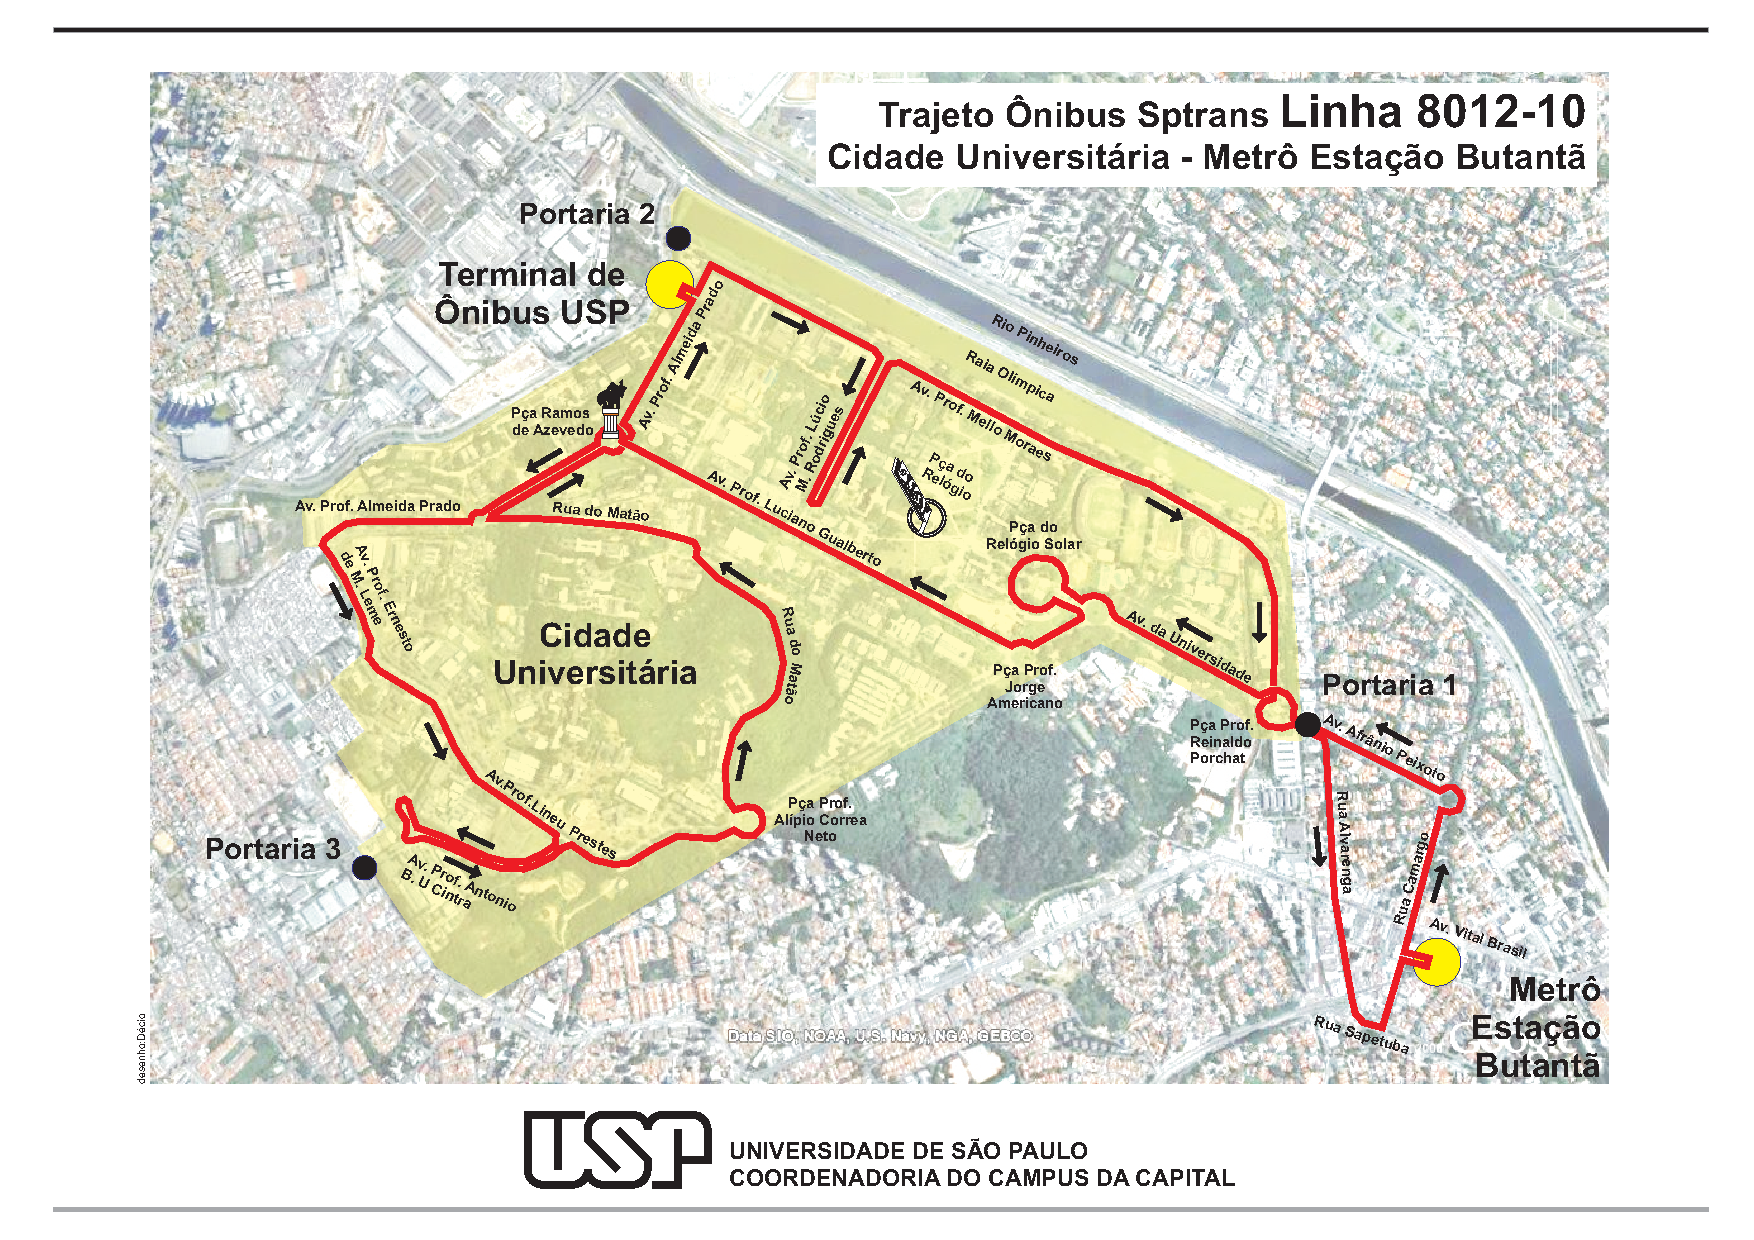
\includegraphics[height=\textwidth, angle=90]{img/8012-10.pdf}
\end{figure}

\begin{figure}[H]
  \begin{center}
    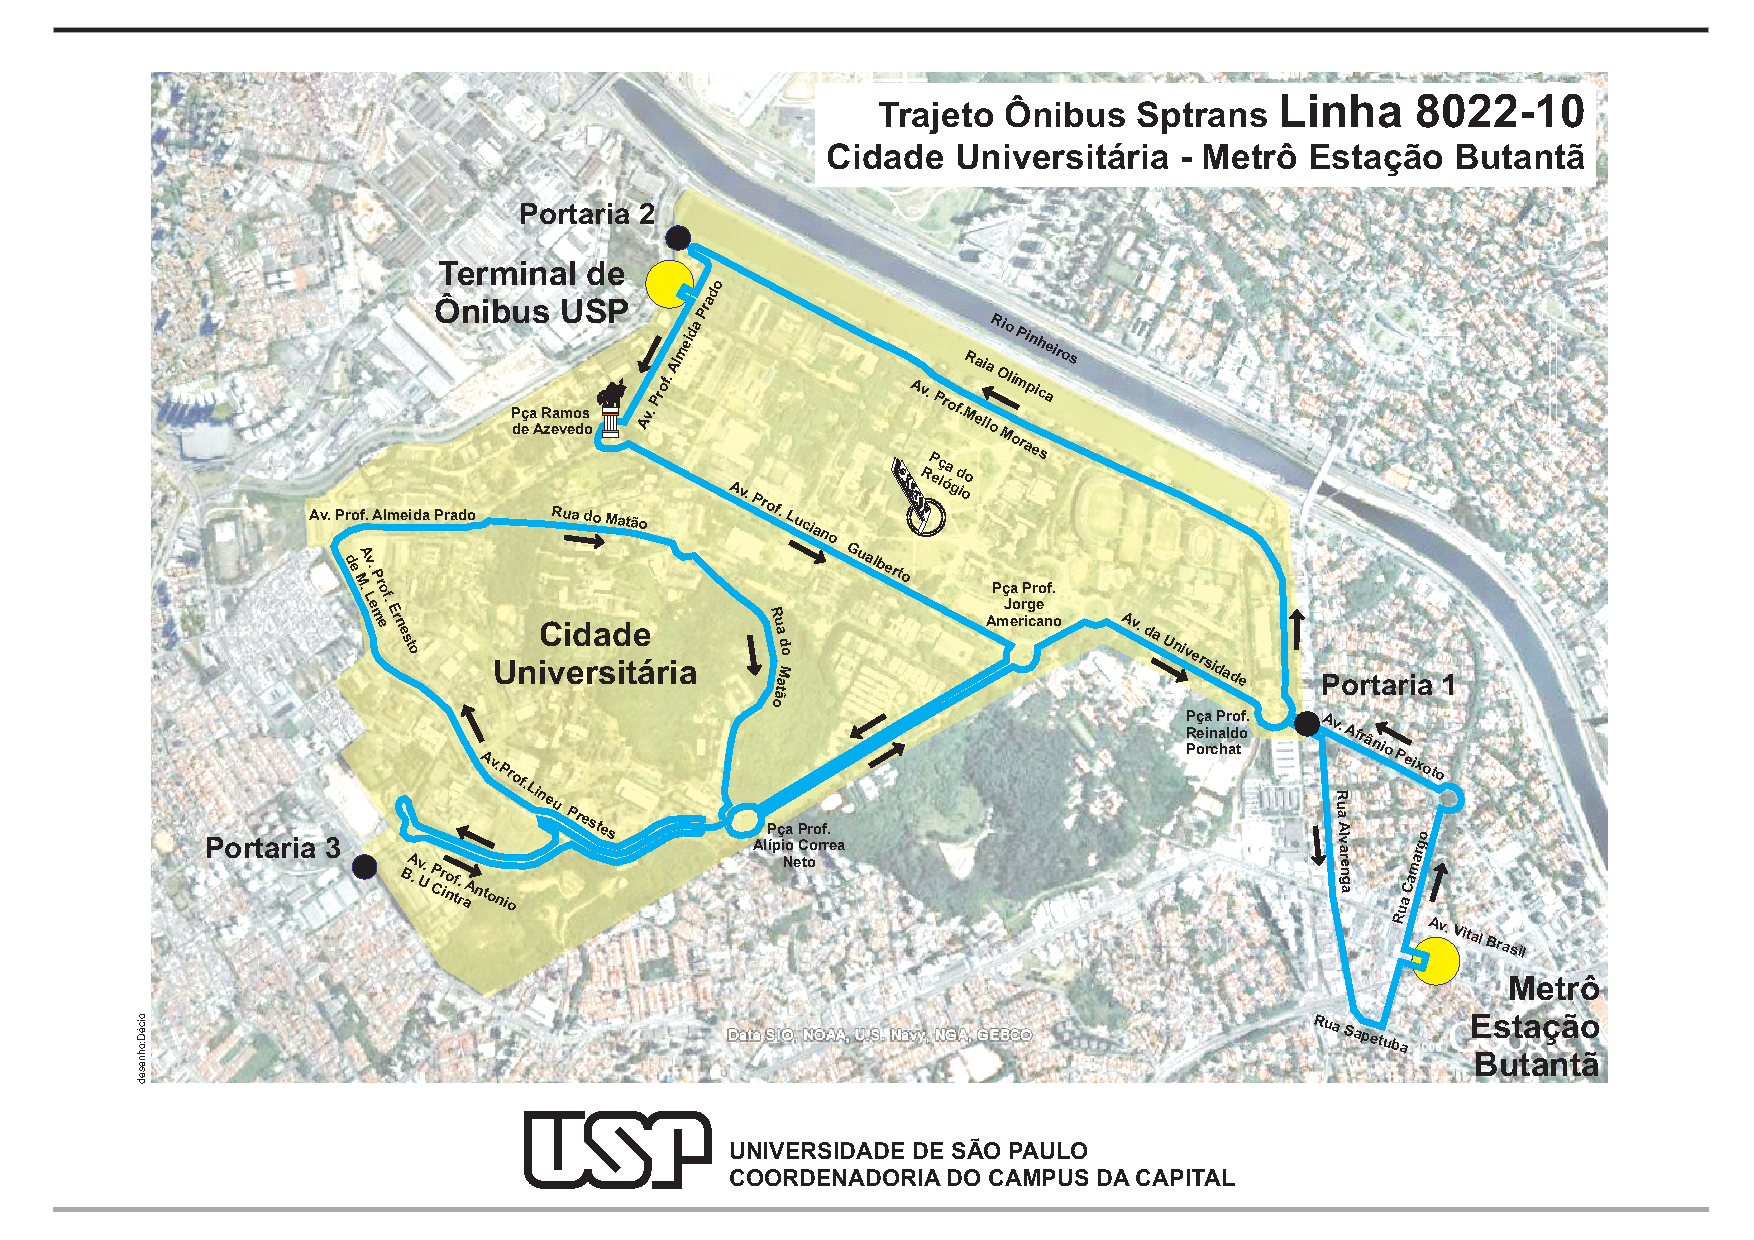
\includegraphics[height=\textwidth, angle=90]{img/8022-10.pdf}
  \end{center}
\end{figure}


\begin{subsecao}{Veículos no Campus}
Saiba por onde entrar na USP. Lembre-se de ter sempre a sua carteirinha USP ou
seu comprovante de matrícula com RG em mãos. 
\begin{itemize}
  \item {\bf Portaria 1 (P1):} R. Afrânio Peixoto. Funciona 24h por dia todos os
    dias, mas a entrada é controlada de segunda à sexta das 20h às 05h, aos sábados
    após as 14h e domingo o dia inteiro. É por onde entram os ônibus municipais. 
    
  \item {\bf Portaria 2 (P2):} Av. Escola Politécnica. Funciona das 5h30 às 20h
    de segunda a sexta. Entrada controlada de seg a sex das 20h às 24h. Fechada
    aos sábados, domingos e feriados. Única entrada para caminhões. 
    
  \item {\bf Portaria 3 (P3):} Av. Corifeu de Azevedo Marques. Tem o mesmo horário
    de funcionamento da P2.

  \item {\bf Portaria 1/2:} R. Eng. Teixeira Soares. Funciona de segunda a sexta das 5h30 às 20h. 
    
  \item {\bf Portarias de pedestre (Mercadinho, São Remo, HU, FEPASA e
      Vila Indiana):} Funcionam de 2ª a 6ª, das 05 às 23 hs.

\end{itemize}

Aos fins de semana, ficam abertas apenas as portarias 1 e 3 (esta, fecha mais cedo). É preciso se identificar.

Os ônibus entram no sábado até as 14h e não entram no domingo. Se você vem de carro, saiba que a universidade dispões de bolsões de estacionamento
gratuito em torno das Unidades.

\end{subsecao}

\begin{subsecao}{Pontos de táxi}
Existem alguns pontos de táxi espalhados pela Cidade Universitária. Eis suas
localidades:

\begin{itemize}
\item Ponto da FEA / ECA (atrás do Banespa)\\
Fone: 3091-4488

\item Ponto da Reitoria\\
Fone: 3091-3556

\item Ponto do Hospital Universitário\\
Fone: 3091-3536
\end{itemize}
\end{subsecao}


\end{secao}


% Dicas ------------------------------------------------------------------------
\begin{secao}{Dicas}

Como todos os bixos são perdidos, aqui vão algumas dicas pra vocês não ficarem perguntando o tempo todo:

%TODO Checar isso aqui.
{\bf Biblioteca:} Para se inscreverem, basta comparecerem à biblioteca munidos do
cartão USP, definitivo ou provisório. O empréstimo é unificado, sendo possível
retirar livros em qualquer uma das bibliotecas da USP mediante apresentação do
cartão USP.

% Não tem mais =(
%{\bf Correios:} tem uma agência em frente à prefeitura do campus.

{\bf Bancos e Caixas Eletrônicos:} Agências do Santander, Bradesco,
Banco do Brasil, HSBC e Itaú na Av. Prof. Luciano
Gualberto; Caixas eletrônicos perto do bandejão da Física, em frente à reitoria,
no CEPE, enfim, em lugares aleatórios.

\begin{subsecao}{Cultura na USP}

{\bf Museu de Arqueologia e Etnologia (MAE):} ao lado da Prefeitura do Campus.

% TODO Descobrir se o MAC está reformando ou será demolido?
{\bf Museu de Arte Contemporânea (MAC):} próximo ao CRUSP.

{\bf Museu do Brinquedo:} fica na Faculdade de Educação, Bloco B.

{\bf Museu do Crime:} na Academia de Polícia perto da P1.

{\bf Museu do Instituto Oceanográfico:} adivinha?

{\bf Museu da Geociências:} Lá mesmo.

{\bf Instituto Butantan:} Próximo à História.

{\bf Museu da Faculdade de Veterinária} Perto do P3. Ponto final do circular.

{\bf Estação Ciência:} fica fora da USP. R. Guaicurus, 1274 - Lapa

{\bf Museu Paulista, vulgo Ipiranga: }também fora da USP, no Parque da
Independência - S/N  - Ipiranga.

{\bf Museu de Zoologia: }também fora da USP, na Av. Nazaré, 481  -
Ipiranga.

{\bf CinUSP Paulo Emílio} Dentro do campus, próximo ao bandejão central, existe uma sala de cinema. Durante todo o ano ocorrem várias mostras cinematográficas, nas quais são exibidos inúmeros filmes. As sessões são gratuitas e a programação pode ser conferida no seguinte site: {\tt http://www.usp.br/cinusp/}


\end{subsecao}

\begin{subsecao}{Onde beber?}

Se você é um dos bixos que curte entornar os canecos de vez em quando, então agora
deve estar pensando, até que enfim vamos falar de algo que presta! Lembre-se de
levar um VETERANO para pagar a ele algumas doses, pois graças a eles que você
está recebendo essas dicas, então sem mais delongas, aqui vão alguns lugares
firmeza para se fazer isso à vontade:

{\bf FAU:} O grêmio da FAU sempre vende cervejas, cada hora uma marca e tamanho diferente. Para chegar, basta ir no primeiro andar à direita até o fim.

{\bf Física:} Embora seja a Física, lá é um lugar gostoso para tomar vários
tipos de cerveja, que só é vendida após as 18:00 horas, e comer alguns
salgados baratos. No próprio C.A. deles se vende cerveja.

{\bf FFLCH:} Vá até o prédio da História e Geografia e procure o Aquário, se estiver alguém lá dentro eles vendem cerveja.

%FIXME Qual é a situação atual do QiB?
{\bf ECA:} Famosa Quinta i Breja, adivinha que dia da semana isso acontece?
Acertou, de quinze em quinze dias nas quintas-feiras, parabéns! bixos que
acertam essa pergunta podem, como prêmio, pagar uma breja para o seu VETERANO
favorito!

{\bf Rei das batidas:} Muito famoso não só por quem estuda na USP, o Rei,
como é carinhosamente chamado, fica fora da USP, saindo pela P1. Vende
diversas batidas e, é claro, cerveja...

{\bf Bar do frango:} Não se sabe qual é o verdadeiro nome desse bar, mas ele é
uma alternativa ao Rei, quando este se encontra muito lotado. Apesar do péssimo atendimento e do aspecto horrível do lugar é bom para beber sem
tumulto. É frequentado principalmente no começo do ano. Se encontra atrás do
Rei.

É claro que também há as festas, que ocorrem em qualquer lugar da USP, e nelas
há ainda outras misturas alcoólicas impossíveis.

É nosso dever informar também que o álcool é uma substância altamente viciante
e, quando bebida em excesso, pode trazer graves consequências à sua saúde, às
vezes à saúde de outra pessoa, à sua família e principalmente ao seu bolso.
Portanto, não se esqueça de abastecer os seus VETERANOS.

\end{subsecao}
\end{secao}


% Melodias para a bixarada -----------------------------------------------------
\begin{secao}{Músicas para a Bixarada}

%\quadrinhos6


\begin{subsecao}{Grito de Guerra da Matemática}

Arakam Baram Bakam / Tumberê tumberá / Macambê mecambecá \\
Rico reco rico rá / Rá rá rá / Matemá matemá Matemá-ti-ca!
\end{subsecao}

\begin{subsecao}{Musiquinha da Poli}

{\em cantar como ``Ele é um bom companheiro''}

Escola de Viadinho \\
Escola de bunda-mole \\
Se é verdade que o mundo tem cu \\
O cu do mundo é a poli  (3x)
\end{subsecao}

\begin{subsecao}{Caboclo da MAT}

{\em cantar como ``Faroeste Caboclo'' da Legião Urbana}
{\em Essa música é em memória a FUVEST, quando Matemática Aplicada e POLI petenciam a mesma carreira}
\begin{verse}
Cheio de medo em setembro Joãozinho viu que seus dedos tremiam pra fazer a
inscrição

Deixou pra trás a namorada, a motoca, o futebol e as festinhas pra rachar na
revisão

Quando criança só pensava em ser engenheiro ainda mais com o dinheiro que
sonhava em ter na mão

Era o CD lá do colégio onde estudava e todo mundo admirava o boletim desse
cuzão

Ia pra igreja só pra rezar pro seu santo pra pedir a sua ajuda pra prestar
vestibular

Sabia mesmo que ia ser barra pesada porque tinha muito japa pra tomar o seu
lugar

O ano todo se propôs a estudar, passava o dia sem ligar a televisão

Nos feriados não ia viajar, ficava em casa treinando redação

Fazia todos os exercícios da apostila e no fim de cada aula ia falar com o
professor

Às quinze horas ia pro laboratório ver as mitocôndrias da aula anterior

Não entendia como o militarismo dominou nosso país por vinte anos de terror

Ficou cansado de tentar achar resposta e desceu pra lanchonete pra afogar a sua
dor

E lá chegando foi tomar um cafezinho e encontrou um concorrente com quem foi
falar

E o concorrente aumentou seu desespero pois manjava muita coisa que ele tinha
que estudar

Dizia ele, eu vou prestar o ITA... Nesse país prova pior não há

E se não der eu vou pegar engenharia, lá na POLI eu vou tomar o seu lugar

E João não gostou dessa proposta, ele disse ``ai que bosta, eu tô passando mal''

Ele ficou bestificado com a idéia de pegar lista de espera só depois do
carnaval

Meu Deus, é pior ainda, no ano novo eu posso estar lá na Mauá

É brincadeira querer ser engenheiro e só descolar emprego em Taguatinga

Na sexta-feira ele morria de vontade de correr pro banheiro se borrando de
pavor

E conhecia muita gente arrogante que passava do seu lado se dizendo um terror

Ele estudava o relevo da Bolívia, função quadrática e modular

E nos domingos então ele fazia tarefa mínima e complementar

E Joãozinho até a morte se esforçava e o tempo mal sobrava pr'ele se alimentar

E via às duas horas o Vestibulando que passava todas as dicas sobre o
vestibular

Mas ele não queria mais conversa e decidiu que em novembro era hora de rachar

Ele pirou que precisava estudar tanto, virou um bitolado e começou a delirar

E logo, logo os malucos da sua idade viram a calamidade, tem babaca novo aí

E o nosso Joãozinho ficou louco e bateu em todos os japoneses dali

Seus amigos preocupados com a sua sorte deram uma fita de rock pr'ele relaxar

Mas de repente sob uma má influência dos boyzinhos lá do fundo começou a zoar

Já na primeira fase ele penou e só passou porque o corte foi sessenta e três

A demência tomou a sua mente : ``Vocês vão ver, eu vou pegar vocês!!!''

Agora Joãzinho era fodido e estava decidido que não ia se dar mal

Sacava toda a trigonometria e manjava de limites, derivada e integral

Foi quando conheceu uma menina e de toda aquela zona ele se arrependeu

Maria Lúcia era uma bitola linda e o coração dele pra ela o Joãzinho prometeu

Ele dizia que devia estudar, pois engenheiro ele queria ser

Maria Lúcia, pra sempre vou te amar, Engenharia com você quero fazer

O tempo passa e um dia chega a hora de fazer segunda fase coitadinho do João

E ele faz uma prova perigosa diz que espera uma resposta, pode ser um sim ou
não

Não vou correndo pra banca de jornal nem pra pátio do cursinho isso eu não faço
não

Pois eu prefiro ficar na minha casa esperando o resultado com o cu na mão

Maria Lúcia vai comprar o tal jornal e logo após achar seu nome ela procura o
de João

Mas ela volta com tristeza no olhar, olha pra ele e diz ``você pegou a quarta
opção''

Você passou na sua quarta opção, você passou na sua quarta opção

Bacharelado em Matemática é um tesão, eu vou sofrer as conseqüências como um
cão

Não é que Joãozinho estava certo, seu futuro era incerto mas foi se matricular

Matriculou-se e no meio da zoeira descobriu que tinha muitos como ele no lugar

Fez inscrição pro remanejamento e talvez no fim do ano transferência ia tentar

E Joãozinho mantinha a esperança de um dia ir pra Poli estudar química

Mas acontece que um tal Professorzzini terrorista de renome apareceu por lá

Ficou sabendo dos planos de Joãozinho e decidiu que com suas notas ele ia se
ferrar

E ele teve que largar cálculo dois mesmo sabendo derivar e integrar

E decidiu deixar estat pra depois que o Moretin voltasse a lecionar

Professorzzini, professor mais sem vergonha com sua prova enfadonha fez todo mundo
dançar

Desvirginava bixetes inocentes e o nabo era tão quente que nem dava pra sentar

E Joãozinho há muito não via sua amada, e a saudade começou a apertar

Eu vou pra Poli eu vou ver Maria Lúcia, já está em tempo de a gente se
encontrar

Chegando à Poli então ele chorou quando viu Maria Lúcia namorando um japonês

Oh, Maria Lúcia, quanto que você mudou, que estrago que a Poli te fez

Joãozinho era só ódio por dentro e então o japonês para um duelo ele chamou

Amanhã às duas horas no biênio, ou na praça do relógio, seja lá onde for

E você pode escolher as suas armas: derivadas ou matrizes de qualquer versor

Que eu provo que o sub-espaço nulo é o coração dessa piranha a quem jurei o meu
amor

E Joãozinho não sabia o que fazer quando escutou um papo lá no bandejão

Onde falavam dum duelo que iam ver dizendo a hora, o local e a razão

No sábado então às duas horas toda a Poli sem demora foi lá só pra assistir

Um japa que botava pelas costas, encoxou Maria Lúcia e começou a sorrir

Sentindo um ódio na garganta João olhou pros cabacinhos e pros trouxas a
aplaudir

E olhou pros pipoqueiros e as bancas de cachorro-quente que passavam por ali

E se lembrou de quando era uma criança e de tudo que vivera até ali

E decidiu entrar de vez naquela dança, se a Poli é um circo, e daí

E nisso o céu abriu seus olhos e então Maria Lúcia ele reconheceu

Ela queria fazer Álgebra dois pra provar que a Poli não a emburreceu

Politécnico, eu sou homem coisa que você não é, e não me contento em por nas
costas não

Some daqui filha da puta sem vergonha vai pra casa tocar bronha o seu destino é
ser bundão

E Joãozinho deu as costas para os dois, foi pra pura onde encontrou o seu valor

Maria Lúcia se arrependeu depois prestou Fuvest mas no IME não entrou

E a todos declarava que o nosso Joãozinho era gênio que escapou de se foder

Que na alta burguesia lá da Poli todo mundo é bunda mole ninguém sabe o que
fazer

E foi dar monitoria no cursinho pra avisar aos molequinhos pra não esquecer

Ele queria era avisar toda essa gente engenharia é pra demente que só quer
sofrer.
\end{verse}
\end{subsecao}

\begin{subsecao}{Musiquinha da Poli 2}

{\em ``A Casa'' de Vinícius de Moraes}

Eu sou viadinho / Eu sou da POLI \\
Meu cu é de ferro / Meu pinto é mole
\end{subsecao}

\begin{subsecao}{Explode Coração}

{\em cantar como ``Explode Coração'' do Salgueiro}

Explode coração / Na maior felicidade / No IME há tanto tempo \\
Sou campeão mas não termino a faculdade
\end{subsecao}

\begin{subsecao}{USP Maravilhosa}

{\em cantar como ``Cidade Maravilhosa''}

Ó USP Maravilhosa / Cheia de encantos mil \\
Ó USP Maravilhosa / Melhor escola do Brasil

Essa é escola que todos querem / Mas poucos conseguem entrar \\
Você que tentou / E não conseguiu \\
Que vá pra puta que pariu!

Ó USP Maravilhosa / Cheia de encantos mil \\
Ó USP Maravilhosa / Melhor escola do Brasil
\end{subsecao}

\begin{subsecao}{Como É Bom Estar no IME}

{\em cantar como ``Que Bonita sua Roupa''}

Como é bom estar no IME \\
Muito bom mas não se anime \\
Já tivemos aula de cálculo \\
Derivada até que é fácil \\
O difícil é integral

Nós somos imeanos \\
Adoramos os queridos VETERANOS \\
Do IME nós gostamos \\
Por aqui nós ficaremos muitos anos
 
Como é bom estar no IME....

Que porcaria é a poli \\
Viadinhos que não gostam de mulher \\
Bando de bundas-moles \\
A menina mais bonita tem bigode

Como é bom estar no IME....
\\
\\
\end{subsecao}
\end{secao}

%\figura{xkcd}

% Utilidades -------------------------------------------------------------------
\begin{secao}{Utilidades}

\begin{subsecao}{Na WEB}

\url{ www.usp.br} - Página da USP. Aqui vocês encontrarão notícias e eventos da
universidade, bem como informações gerais.

\url{ www.ime.usp.br} - Página do IME.
Nesse link, vocês poderão ver detalhes sobre os cursos e obter informações sobre
a faculdade.

\url{ uspdigital.usp.br/jupiterweb} - Sistema JúpiterWeb. Aqui vocês vão
encontrar a grade horária e, mais tarde, vocês poderão fazer as matrículas nas
matérias que irão cursar no semestre, além de ter acesso às suas notas.

\url{ paca.ime.usp.br} - É bixes... acham que vai ser essa moleza pra sempre? Se
vocês acham, estão muito enganados! Daqui a pouco vocês vão receber uma senha para
poder enviar seus EPs (vide glossário) nesse endereço... (e não adianta fazerem
chantagem emocional que o Paca só vai aceitar até 23h55... não entendeu? vocês
vão entender...)

\url{ fb.com/SpottedImeUsp} - Viu alguém interessante? Quer mandar uma cantada
pro crush mas tem vergonha? Manda um spotted! Afinal, só o x deve ficar isolado.

% \url{ www.xkcd.com} - Webcomic sobre matemática e computação. Origem de muitas
% piadas que vocês ouvirão por aí.

E por fim..

\url{ www.google.com.br} - Tudo o que vocês precisam tá no google. Se não estiver,
então não existe. Aproveitem e procurem o Código de Ética da USP (ou baixem ele em
\url{http://www.prg.usp.br/wp-content/uploads/CodigoEtica.pdf})

\end{subsecao}

\begin{subsecao}{Apps}
Apps disponíveis na AppStore e PlayStore oferecidos pela própria USP que podem ajudar. lista completa em: \url{sti.usp.br/appusp}

{\bf Campus USP} - Acesso a central da Guarda Universitária diretamente no caso de uma emergência. Contém mapa com as ocorrências recentes de segurança. 

{\bf Cardápio USP} - Contém o cardápio dos bendejões, além de avisar se o bandejão está fechado ou com horário reduzido.

{\bf E-card USP} - Esse é o app mais importante nesse começo de ano, enquanto sua carterinha não chega (ver seção Cartão USP em júpiter), o aplicativo é uma carteirinha virtual que te da acesso a tudo que a carteirinha física permite, inclusive comer no bandejão.

{\bf Disque-Trote USP} - Use esse app para denunciar caso sofra um trote violento. Se
preferir, também pode ligar para o número de telefone que está logo aqui embaixo.

\end{subsecao}

\begin{subsecao}{Telefones}
Colocamos essa seção aqui apenas para que vocês, bixes, não nos encham com perguntas
sobre passes e plantão:

{\bf SAS:} Seção de Passe Escolar: {\tt 3091-3581}

{\bf Seção de Alunos:} {\tt 3091-6149}

{\bf Disk Trote:} {\tt 0800-012-090} -- \underline{Não deixe de ligar se você sofrer algum trote violento!!}

%{\bf Plantão de Cálculo e Álgebra Linear (serviço gratuito):} {\tt 3037-1773}
%Diziam que era o orelhão do ime, vai que isso volta, resolvi só comentar^^

\end{subsecao}
\end{secao}


% Glossário --------------------------------------------------------------------
\begin{secao}{Glossário}

Esta parte é, sem dúvida, uma das mais importantes do guia. Aqui você
encontrará todas as explicações para as maiores dúvidas do universo. Com
certeza, após ler este trecho sua vida vai mudar: você saberá, por exemplo,
porque o céu é azul e com quantos paus se faz uma canoa.

\begin{subsecao}{Sobre o IME}
{\bf Armários:} Ficam na sala 18 do bloco B (sala da Vivência). Além de
servirem para aliviar imeanos do excesso de peso dos livros e cadernos, ajudam
o CAMAT a sobreviver financeiramente.

{\bf Banheiro:} Temos vários e de três tipos: para Homens, para Mulheres e os
matinhos para os bixos. Recentemente foram reformados os três tipos, então você
bixo, poderá usufruir de um matinho totalmente novo!

{\bf Bichinho esquisito:} Aquele negócio que está nas camisetas, agasalhos e
bonés do IME. Alguns dizem que é o mascote da Atlética; alguns o chamam de
Fluffy; ninguém sabe dizer o que ele realmente é, mas apareceu depois que
surgiram aquelas bolinhas, estilo porco-espinho, feitas com elásticos
coloridos (você provavelmente deve lembrar; foi mais ou menos na época do seu
primário). Primo do Cariboo.

{\bf CEC:} É a sigla do Centro de Ensino de Computação. É um dos lugares onde o
bixo pode fazer (ou pelo menos tentar) seus EP's e onde são ministrados cursos
de Computação para alunos de toda USP (e até de fora).

{\bf GRECIME:} É o grêmio dos funcionários. Portanto quando ouvir falar em
grêmio não pense CAMat. Não tem nada a ver. Fica ao lado do Xerox e é o único
lugar que vende comida no IME desde que o Sandrão foi fechado. O serviço é péssimo
e as chances são que, se você pretende comer por lá durante o intervalo entre as
aulas, não vai dar tempo de ser atendido (uma fila de 5 alunos já demora em torno
de 20 minutos) e você vai logo perceber que vale mais a pena ir até a FAU ou o IO
do outro lado da praça para comprar um salgado.

{\bf IMEJr:} Empresa administrada pelos alunos do IME.

{\bf RD:} Representante Discente. É aquele aluno que representará você nas
comissões do IME, Comissões de Curso, Comissão de Graduação, entre outras.
Nestas comissões serão tomadas decisões que irão influenciar a sua vida
acadêmica. Então a presença de um aluno nelas é imprescindível, pois nada
melhor que um aluno para saber das necessidades dos alunos.

{\bf Sala das ET's:} É uma sala no bloco A onde estão as Work
Stations (Estações de Trabalho), usadas pelos professores, alunos de
pós-graduação e de iniciação científica.

{\bf Sala da Vivência:} É a sala 18 do bloco B, a sala mais importante de todas
do IME e onde os alunos aproveitam para jogar cartas, sinuca, pebolim, xadrez,
fliperama, Pokémon, Magic, ouvir música, assistir TV, dormir no sofá, e o que
mais der na telha de quem quiser relaxar.

{\bf Seção de Alunos:} Aquele lugar onde você faz matrícula (aliás, você deve ir
confirmar a matrícula logo, bixo!), declaração, requerimentos, etc. (assuntos
burocráticos). Vá até o saguão à esquerda do Bloco B (lá onde fica o CEC) entre
na fila. O horário de funcionamento é meio restrito, então não deixe as coisas
pra última hora.

{\bf Xerox:} A Xerox fica entre a Vivência e o Grecime, ou virando à direita logo
depois do balcão de informações no bloco B.

\end{subsecao}

\begin{subsecao}{Sobre as matérias}

{\bf Teorema:} Um teorema é uma afirmação que pode ser provada. Provar
teoremas é a principal atividade dos matemáticos. Deles surgem Lemas,
Corolários, Proposições, e tantas outras coisas que você só vai entender
completamente o que significam quando precisar escrever sobre eles, o que vai
acontecer logo logo!

{\bf Iniciação Científica:} grupo de alunos, coordenado por um professor, que
estuda um determinado assunto, paralelamente ao curso. No caso de alunos que
queiram bolsas de estudo, é adotado um plano de estudos mais rigoroso.

{\bf SUB:} prova que você faz quando vai mal em alguma outra avaliação, ou
quando você simplesmente não vai. Sua aplicação e utilidade depende do
professor ministrante

{\bf REC:} prova que você faz quando vai mal na SUB.

{\bf DP:} matéria que você faz quando vai mal na REC.
\end{subsecao}

\begin{subsecao}{Sobre programas}

{\bf Computador:} objeto com vontade própria, sensível, que requer muito
carinho e atenção. Normalmente comparado às mulheres, com duas pequenas
diferenças: ele faz direito o que você pede e neles podemos fazer upgrades
quando quisermos.

{\bf EP:} Exercício-Programa. Algo que você vai ter que fazer muitas vezes, e
vai dar muito trabalho.

{\bf GCC:} compilador mais recomendado para seus EP's, por suas inúmeras
qualidades. Atenção: ele ainda fará você se sentir burro.

{\bf Hello World:} Um clássico da programação universal.

{\bf Segmentation Fault:} Efeito computacional aleatório causado pela ``véspera
de entrega de EP''. Desenvolvido por Murphy.

{\bf Stack Overflow:} mensagem que aparece na tela do computador
quando ele se recusa a funcionar. Isso ocorre quando ele está magoado, cansado,
ou simplesmente está ``naqueles dias''.

{\bf Teorema Fundamental do EP:} ``O EP só funcionará no dia da entrega.'' Não
confunda com o Corolário 42 da Lei de Murphy: ``O EP só {\bf não} funcionará no
dia da entrega!''

{\bf Linux:} Sistema operacional criado totalmente em linguagem C, graças a um
esforço mundial de milhares de programadores e experts em informática, composto
por aproximadamente 7 mil arquivos e 5 milhões de linhas, e com o qual você não
tem capacidade para trabalhar.

{\bf Windows:} Vírus. Porém tão bem mascarado que parece até a coisa correta a
se usar.
\end{subsecao}

\begin{subsecao}{Sobre a fauna da USP}

{\bf politécnico:} Podemos defini-los através de seu próprio hino: ``Mulher,
mulher pra quê / eu quero a HP; Mulher, mulher que nada / eu quero a derivada;
Mulher, mulher faz mal / eu quero a integral...''

{\bf VETERANO:} O ser supremo. O senhor de sua vida imeana. Nunca responda,
desrespeite, agrida, afronte ou encare um VETERANO. Se um VETERANO lhe dirigir
a palavra agradeça ao seu Deus, pois você foi abençoado. Com todas as letras
maiúsculas e sempre em fontes TrueType.

{\bf Monitor:} VETERANO que é mal pago pelo instituto para tirar dúvidas e
corrigir listas de exercícios e/ou EP's de uma determinada matéria.

{\bf Formado:} VETERANO + diploma

{\bf Mestre:} VETERANO + diploma + dissertação

{\bf Doutor:} VETERANO + diploma + dissertação + experiência + tese

{\bf Professor:} Aquele que sabe muito, só não conta pra você. A maior parte
não fala português; alguns apenas emitem ruídos estranhos.

(N.do E.): Como vocês podem perceber, o VETERANO está em todas. Portanto, você
deve se esforçar ao máximo para se tornar um de nós (esperamos realmente que
você consiga, pois não vai ser fácil)

{\bf bixo:} O ser mais inferior da face da Terra. Para encontrar um basta olhar
no espelho. Sempre em minúsculas.
\end{subsecao}

\begin{subsecao}{Sobre a USP}

{\bf Bandejão:} Local de torturas diárias. Ali você irá receber a sua dose de
substâncias estranhas. Se você criar o hábito de comer lá todos os dias, quando
houver guerra biológica ou radioativa você estará imune.

{\bf CEPE:} Centro de Práticas Esportivas - lugar onde você poderá praticar
todos os esportes que quiser.

{\bf Circular:} ônibus interno da USP. Pegue um (se passar) e conheça a
universidade toda. Dizemos TODA, porque esse ônibus dá voltas incríveis. Por
outro lado, é incrivelmente mais barato que os ônibus da prefeitura, diriamos
até que é o preço que vale andar com tal opção (ou falta dela).

{\bf COSEAS:} ao lado da praça do relógio. É onde os alunos fazem a carteirinha
de passes de ônibus, EMTU e metrô, além de solicitar os auxílios eteceteras que
estão explicados na seção respectiva.

{\bf CRUSP:} Conjunto residencial da USP. Se você se inscrever, torça para
pegar um apartamento num dos blocos já reformados, ou então torça para não
conseguir nenhum.

{\bf Colméia:} conjunto de favos.

{\bf Favos:} um monte de prédios hexagonais encravados no meio do CRUSP.

{\bf CINUSP:} Cinema da USP localizado no favo 4 da Colméia. Toda semana ele
passa um filme de qualidade. Informe-se sobre a programação em {\tt www.usp.br/cinusp}

{\bf Pelletron:} prédio da Física que na realidade é um acelerador de
partículas. Nada de ter idéias mirabolantes, Joselito...

{\bf PUTUSP:} Se você, bixo, quiser fazer Iniciação (não científica), vá até a
Avenida Valdemar Ferreira (saída principal da USP). Lá estarão os(as)
instrutores(as) dispostos a iniciá-lo 24 horas por dia.

{\bf Vet (Veterinária):} Para onde são mandados os bixos que se machucaram no
trote.

{\bf H.U. (Hospital Universitário):} para onde são mandados os bixos que não
foram aceitos na Vet. Lá são realizados os tratamentos e experiências com
exposição a radiação, exposição a aspirantes a médicos, teste de
paciência/resistência a dor assim que pega a senha, alto nível de gesso no
estômago, queda espontânea (ou não) de cabelo etc.

{\bf Psico:} Para onde mandamos os bixos que pensam que são gente.

\end{subsecao}
\end{secao}


% Considerações Finais ---------------------------------------------------------
\begin{secao}{Considerações Finais}

Este guia chegou ao fim. Vocês devem estar pensando ``E agora? O que nós, bixes,
vamos fazer, sozinhos nessa faculdade?''

Se precisarem de alguma ajuda, basta procurarem algum veterane, que ele te
ajudará (provavelmente ele também não saberá a resposta, mas talvez conheça
alguém que saiba).

Não esqueçam de comprar seu kit-bixe para ajudar a Comissão e tornar a recepção
do ano que vem mais legal que a de vocês. Participem da Semana de Recepção,
carinhosamente preparada pelo Instituto e pelos seus veteranes devidamente
identificados. Último conselho: guardem este guia para o resto de sua graduação.
Por mais ``veteranes'' que sejam, vocês precisarão dele.

Sugestões, elogios, presentes, bajulações ou quaisquer outras coisas para a
Comissão podem ser enviadas para: \url{https://www.facebook.com/recepcaoimeusp}

Se vocês encontraram algum dos vários erros espalhados como exercício pelo texto,
nos enviem uma mensagem no Facebook, ou \textbf{participem da Comissão no ano que vem}
e ajudem vocês também na próxima edição do Guia do Bixe!

\end{secao}


\end{document}


